%%%%%%%%%%%%%%%%%%%% author.tex %%%%%%%%%%%%%%%%%%%%%%%%%%%%%%%%%%%
%
% sample root file for your "contribution" to a contributed volume
%
% Use this file as a template for your own input.
%
%%%%%%%%%%%%%%%% Springer %%%%%%%%%%%%%%%%%%%%%%%%%%%%%%%%%%


% RECOMMENDED %%%%%%%%%%%%%%%%%%%%%%%%%%%%%%%%%%%%%%%%%%%%%%%%%%%
\documentclass[graybox]{svmult}
\usepackage{svmult}
% choose options for [] as required from the list
% in the Reference Guide

\usepackage{mathptmx}       % selects Times Roman as basic font
\usepackage{helvet}         % selects Helvetica as sans-serif font
\usepackage{courier}        % selects Courier as typewriter font
\usepackage{type1cm}        % activate if the above 3 fonts are
% not available on your system
%
\usepackage{makeidx}         % allows index generation
\usepackage{graphicx}        % standard LaTeX graphics tool
% when including figure files
\usepackage{multicol}        % used for the two-column index
\usepackage[bottom]{footmisc}% places footnotes at page bottom

\usepackage{amsmath}
\usepackage{amssymb}
\graphicspath{{./figs/}}
\usepackage{bm}

\usepackage{algorithm}
\usepackage{algorithmic}
%\usepackage{subcaption}
\usepackage{relsize}
\usepackage{url}

% see the list of further useful packages
% in the Reference Guide

\makeindex             % used for the subject index
% please use the style svind.ist with
% your makeindex program

%%%%%%%%%%%%%%%%%%%%%%%%%%%%%%%%%%%%%%%%%%%%%%%%%%%%%%%%%%%%%%%%%%%%%%%%%%%%%%%%%%%%%%%%%

\begin{document}
	
	\title*{Graph-based Wavelet Multiresolution Modeling of Multivariate Terrain Data}
	% Use \titlerunning{Short Title} for an abbreviated version of
	% your contribution title if the original one is too long
	\author{Teodor Cioac\u a and Bogdan Dumitrescu and Mihai-Sorin Stupariu}
	% Use \authorrunning{Short Title} for an abbreviated version of
	% your contribution title if the original one is too long
	\institute{Teodor Cioac\u a \at \email{t.cioaca@gmail.com}
		\and Bogdan Dumitrescu \at University Politehnica of Bucharest \email{bogdan.dumitrescu@acse.pub.ro}
		\and Mihai Sorin-Stupariu \at University of Bucharest \email{stupariu@fmi.unibuc.ro}}
	%
	% Use the package "url.sty" to avoid
	% problems with special characters
	% used in your e-mail or web address
	%
	\maketitle
	
	\abstract{Terrain data pose modeling challenges due to their high inherent redundancy and difficulty of identifying features at different levels of detail. We propose a multiresolution analysis framework based on a graph-based wavelet construction. Our approach produces a sequence of intermediate resolution approximations of the terrain model. The details pertaining to each resolution reveal scale-specific features. Using a guiding heuristic, the proposed wavelet construction also conserves salient features. Furthermore, the proposed framework allows both geometric and attribute vertex information and can be used for modeling tasks sharing the same characteristics and constraints with terrain modeling. In particular, our graph-based wavelet framework is an option for multiresolution filtering and feature classification or clustering.}
	
	\section{Introduction}
	\label{sec:1}
	
	The particular problematics of terrain modeling span a broad range of quantitative and qualitative analysis tasks. Such tasks include, but are not limited to geometric representation, geomorphological feature identification and analysis, vegetation coverage analysis and extraction. The continuous advancements of 3D sensor scanning technologies and the increasing popularity of civil aerial drones further facilitate gathering high density point cloud 
	terrain representations. 
	
	In this chapter, we describe an approach for multiresolution analysis of multivariate terrain data, which is also suitable for other data organized in similar structures. In general, the framework we propose can be easily adapted for performing multiresolution analysis on triangulated point clouds, meshes or graphs. Any of these data structures may describe an irregular domain where a multivariate signal is discretized. These samples are then concentrated in the vertices of these structures.
	
	Given these aspects, the approach we will further describe capitalizes on recently developed methods for graph signal processing. More specifically, we explore a wavelet-based graph multiresolution construction having a reduced approximation error and is computationally efficient. The graph wavelet interpretation facilitates tasks involving \emph{vertex frequency analysis} or \emph{multiresolution filtering and clustering}.
	
	
	\subsection{Terrain data representation}
	Typically, the geometric information describing terrain fragments is encoded in a
	digital elevation model (DEM) \cite{vanKreveld1997}. A triangulated irregular network (TIN) is a further
	specialization of a DEM where both point and primitive (triangle) sampling is allowed to be irregular,) reducing the highly redundant mation in flat (inf regions.
	De Floriani and Magillo \cite{Floriani2016} provide the following definition:
	
	\begin{quotation}
		A terrain can be mathematically modeled as a function $z = f (x, y)$ mapping a point $(x, y)$ in a domain $D$ in the plane to its elevation value $f (x, y)$.
		In practice, the value of function $f$ is known on a finite set $S$ of points within $D$. 
		A DEM provides an estimated value for function $f$ at any point $(x, y)$ of the domain, based on the values at the points of $S$. 
		A DEM consists of a subdivision of the domain into cells and of a piece-wise interpolating function defined on such cells.
		A TIN is a DEM in which the domain subdivision is a triangular mesh, i.e., a set $T$ of triangles such that: 
		\begin{enumerate}
			\item the set of vertices of $T$ is $S$
			\item the interiors of any two triangles of $T$ do not intersect
			\item if the boundaries of two triangles intersect, then the intersection is either a common vertex, or a common edge.
		\end{enumerate}
	\end{quotation}
	
	We can easily conclude that the TIN definition is practically identical to that of a triangular mesh as generally understood in the field of Computer Graphics.
	
	
	\subsection{Challenges of terrain modeling from raw point data}
	LiDAR data are usually dense and the information richness can pose a problem on its own since there is no intrinsic manner of reducing geometric or other attribute redundancy.
	However, model simplification is a well studied problem for which established solutions have been proposed in the field of Computer Graphics. Among the computationally efficient
	approaches, we mention \emph{incremental thinning}, where geometric primitives are simply removed by following a local quality-based simplification criterion. For TIN models,
	Demaret et al. \cite{Demaret2005} have proposed an efficient coarsification algorithm via incremental point removal.
	
	Suarez and Plaza \cite{Suarez2009} have introduced a coarsening algorithm applicable to RTINs (right-triangulated irregular networks). Their method is especially efficient
	given that both the underlying geometry and triangle primitive connectivity is easier to control than in the case of general irregular networks as each vertex has a maximum of
	8 directly connected neighbors. The actual coarsening is then achieved through edge midpoint split operations, which are also invertible.
	
	Another problem posed by raw point clouds is that there is no immediate and accurate information concerning the ground or vegetation class of constituent points.
	While ground return information can help define a subset of soil-level points, the overall point cloud usually contains more ground-level information, as well as potentially
	unclassified data points.
	Evans and Hudak \cite{Evans2007} have designed a \emph{multiscale curvature classification algorithm} (MCC) in order to filter and classify points present in raw LiDAR collections.
	
	Silva et al. \cite{Silva2018} examine four different algorithms for classifying ground from hovering points in point cloud terrain data sets. Among the algorithms discussed 
	in their work, the Progressive Triangulated Irregular Network (PTIN), implemented in the LAStools package \cite{Isenburg2015}, was proven to possess good performance characteristics
	(low RMSE and increased ground classification accuracy with respect to the ground truth). 
	
	
	\subsection{Existing solutions}
	Given that terrain modeling tasks pose similar problems to those encountered in point cloud, mesh or graph data processing, we will briefly review some of the milestone achievements from these areas.
	
	\subsubsection{Incremental simplification of point clouds and meshes}
	Historically, solutions to feature redundancy have been addressed separately from multiresolution analysis. The most common solution to this problem is incremental simplification. Modeling of terrain data is also possible with either point cloud or mesh simplification methods.
	
	For point clouds, notable contributions are given in the work of
	Pauly et al.  \cite{Pauly2002} where three simplification method categories are detailed: clustering, iterative simplification and particle simulation.
	
	In the case of triangular or polygonal meshes, the additional information
	also facilitates the creation of reversible, continuous level-of-detail representations and mesh morphing. Schroeder et al. \cite{Schroeder1992} were among the first authors to discuss triangular mesh simplification in a step-by-step manner known as \emph{decimation}. Almost all decimation-based methods require the existence of a decimation criterion and can be summarized in two steps that are repeated until the target density is reached:
	\emph{(i)} evaluate decimation criterion (usually a cost function estimating the impact of removing a set of primitives) and \emph{(ii)} remove a primitive and re-triangulate the local geometry.
	
	To address changes in the mesh connectivity resulting from primitive removal, Ronfard et al. \cite{Ronfard1996} proposed a reversible operation called \emph{edge collapse}. One of the most effective heuristic criteria for guiding these operations is the \emph{quadric error metric} formulation of Garland and Heckbert \cite{Garland1998}.
	
	\subsubsection{Wavelet multiresolution methods}
	Successful initiatives for adapting established Signal Processing methods for
	point cloud, mesh and graph analysis have been recorded. 
	
	To briefly summarizes notable adaptations of wavelet-like transforms on point clouds we mention the following works. Chen et al. \cite{Chen2010} have introduced an SVD-based construction of so-called geometric wavelet point cloud analysis. Earlier, Choi et al. \cite{Choi2005} applied a straightforward implementation of Swelden's \emph{lifting scheme} \cite{Sweldens1996} for denoising point sampled manifolds of low intrinsic dimension.
	
	Among the first wavelet mesh multiresolution analysis methods is that of Lounsbery \cite{Lounsbery1994}. Using a subdivision operator on triangular meshes, Lounsbery introduced an analog of the refinement equation for functions defined on mesh structures instead on the real line. With the introduction of Swelden's \emph{lifting scheme} \cite{Sweldens1996}, other approaches using this technique were developed. One example is the critically sampled design for irregular meshes described by Bertram \cite{Bertram2007}. His method is similar to that of Guskov et al. \cite{Guskov1999}, where a geometry-based subdivision operator defines wavelet synthesis.
	
	After mesh wavelet constructions, algorithms specifically design for more generic graph data were also introduced. We mention the method of Coifman et al. \cite{Coifman2006}, which uses a diffusion operator to build a wavelet transform in the graph frequency domain. Hammond et al. \cite{Hammond2011} further proposed a method that, instead of diagonalizing the graph Laplacian matrix, a costly process for large graphs, uses approximations based on Chebyshev polynomials. In the graph spatial domain we mention Jansen's approach \cite{Jansen2001, Jansen2013}, also adopted and extended by Wagner et al. \cite{Wagner2005}, and by Martinez and Ortega \cite{Martinez2011}.
	
	\subsubsection{Wavelet multiresolution for terrain modeling}
	Among the first solutions specifically designed with terrain modeling in mind is the \emph{wavelet triangular irregular networks} framework of Wu and Amaratunga \cite{WuA03}. This method is essentially a \emph{lifting scheme} adaptation using an inverse subdivision prediction filter and resampling in the $xy$ plane. The importance of wavelet coefficients, byproducts of multiresolution analysis, was emphasized by Beyer \cite{Beyer2003}. The author demonstrated that both terrain gradient and curvature information can be derived from these wavelet detail vectors. Kalbermatten's et al. \cite{Kalbermatten2012} work further explores applications of wavelet transform in identifying multiscale geomorphological and geological features.
	
	\section{Terrain modeling using graph-based wavelet multiresolution analysis}
	We now address the question of how a wavelet multiresolution framework can be defined for terrain models. From a signal processing perspective, DEMs are similar to images, which are simply two-dimensional signals defined over regular domains. When modeling data from LiDAR sources, TIN structures are better options because they allow for adaptive sampling in areas with high geometric redundancy. Building wavelets on these irregular domains would enable the analysis of terrain characteristics at different levels of 
	resolution, which, in turn, can be perceived as information pertaining to a certain frequency band.
	
	Our goal is threefold. First, we aim to expand previous methods and achieve multiresolution representation of multivariate terrain sets (having both geometric and attribute coordinates for each point). Second, by adopting a spatial domain graph lifting scheme construction, we maintain a balance between computational complexity and the range of potential practical applications of the method. Third, we wish to explore the semantic interpretation of detail vectors, leading to a correlation between vertices and levels of resolution. This interpretation would allow our method to be applicable to \emph{vertex frequency analysis} tasks.
	
	Both the construction and results presented in the following sections of this chapter have been partially described in our previous works \cite{Cioaca2015} and  \cite{Cioaca2016}.
	
	\subsection{Classic wavelet analysis and synthesis}
	Before detailing our wavelet multiresolution design for multivariate signals, we review the fundamental concepts in the one-dimensional case.
	%%%%
	\subsubsection{Problem formulation}
	In general, wavelets are the building blocks of hierarchical function space approximations, i.e. $L^2(\mathbb{R}) \succ \ldots \succ V_n \succ V_{n-1} \succ \ldots \succ V_{1} \succ V_{0} \succ \ldots \succ \{0\}$, where $V_{j}$ is a function space approximation at level $j$. We are interested in examining the connections between two consecutive approximations, $V_{j+1}$ and $V_{j}$. Let $\Phi_j = \begin{bmatrix} \ldots & \phi_{j,k} & \ldots \end{bmatrix}$ be the row vector of basis functions that generate $V_j$. Then a function $f_{j+1} \in V_{j+1}$ cannot be represented by using only the basis functions in $V_{j}$, but it can be expressed as a combination of the basis functions of the $V_{j+1}$ space, that is
	\begin{equation}
	f_{j+1} = \Phi_{j+1} \mathbf{s}_{j+1},
	\label{eq_cds:f_in_j_plus_one}
	\end{equation}
	where $\mathbf{s}_{j+1}$ is an infinite column vector of \emph{scaling coefficients}. The  complementary basis or \emph{wavelet functions}, $\psi_{j,k}$, that generate the orthogonal subspace, $W_j$, with $V_{j+1} = V_j \oplus W_j$, correspond to the lost details. One can hence write
	\begin{equation}
	f_{j+1} = \Phi_{j+1}\mathbf{s}_{j+1} = \Phi_j \mathbf{s}_j + \Psi_j \mathbf{w}_j,
	\label{eq_cds:f_in_j}
	\end{equation} 
	where $\Psi_j = \begin{bmatrix} \ldots \psi_{j,k} \ldots \end{bmatrix}$ and $\mathbf{w}_j$ is the infinite column vector of \emph{wavelet coefficients}.
	
	
	Both the scaling and wavelet coefficients can be written in terms of internal products between $f_{j+1}$ and the dual basis functions of their corresponding spaces, i.e.:
	\begin{eqnarray}
	\mathbf{s}_{j+1,k} & = & \left< \tilde{\phi}_{j+1,k}, f_{j+1} \right>,
	\label{eq_cds:inner1}\\
	\mathbf{s}_{j,k} & = & \left< \tilde{\phi}_{j,k}, f_{j+1} \right>, \label{eq_cds:inner2}\\
	\mathbf{w}_{j,k} & = & \left< \tilde{\psi}_{j,k}, f_{j+1} \right>.
	\label{eq_cds:inner3}
	\end{eqnarray}
	
	%%%%
	
	\subsubsection{Second generation wavelets}
	Let $\mathbf{x} = (x_k)_{z\in \mathbb{Z}}$ be an infinite sampled signal.
	
	The first operation involved in the lifting procedure is called a \emph{split} or \emph{parity assignment}. To this effect, the signal is divided into two sets, an even set, corresponding to $\mathbf{x}_e = (x_{2k})_{k\in \mathbb{Z}}$ and an odd set, corresponding to $\mathbf{x}_o = (x_{2k+1})_{k\in\mathbb{Z}}$.
	
	The second operation of the lifting procedure is the \emph{prediction step}. This implies approximating the odd samples using the even ones by applying a prediction operator, $\mathbf{P}$, i.e.
	\begin{equation}
	\mathbf{d} = \mathbf{x}_o - \mathbf{P} \mathbf{x}_e,
	\end{equation}
	obtaining the signal $\mathbf{d}$ of \emph{approximation errors} or \emph{detail coefficients}.
	
	
	\begin{figure}[t]
		\centering
		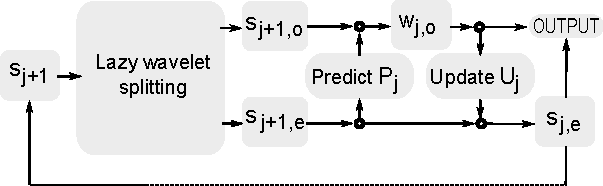
\includegraphics[width=\textwidth]{lifting_diagram}
		\caption{The \emph{lifting scheme} diagram: Splitting (equation (\ref{eq_cds:lifting_splitting})) is followed by prediction via equation (\ref{eq_cds:coeff_predict}) and then by the updating of the low resolution output via equation (\ref{eq_cds:coeff_update}).}
		\label{fig_cds:lifting_diagram}
	\end{figure}
	
	
	Usually, the even and odd sample subsets are highly correlated, and, as a direct consequence, it becomes more efficient to store the signal using the information in $\mathbf{d}$ as it has lower entropy than $\mathbf{x}_o$. The prediction phase is equivalent to mapping $(\mathbf{x}_e, \mathbf{x}_o) \to (\mathbf{x}_e, \mathbf{d})$. Since $\mathbf{x}_e$ is essentially obtained through a na\"ive downsampling of the original signal, aliasing occurs and must be appropriately dealt with. This is performed through a third operation, the \emph{update} or \emph{smoothing} phase. Algebraically, this operation is implemented as
	\begin{equation}
	\mathbf{s} = \mathbf{x}_e + \mathbf{U}\mathbf{d},
	\end{equation}
	where $\mathbf{s}$ is the smoothed downsampled signal and $\mathbf{U}$ is the update operator. 
	
	Assembling the \emph{three stages} of the lifting scheme into a sequence, we obtain the flow diagram shown in figure \ref{fig_cds:lifting_diagram}. The flow allows cascading the resulting filter bank by feeding the even output from one lifting pass to the input of another one, effectively creating a series of coarser approximations of the original signal.
	
	Another immediate property of the lifting design is the straightforward invertibility, i.e.
	\begin{eqnarray}
	\mathbf{x}_e &=& \mathbf{s} - \mathbf{Ud} \\
	\mathbf{x}_o &=& \mathbf{d} + \mathbf{P}\mathbf{x}_e.
	\end{eqnarray}
	
	Returning to the function space context, we review the mechanism behind the lifting scheme. The first operation, the \emph{split}, when applied to the set of scaling coefficients at level $j+1$ produces a vector of scaling coefficients reindexed such that
	\begin{equation}
	\mathbf{s}_{j+1} = \begin{bmatrix} \mathbf{s}_{j+1,o} \\ \mathbf{s}_{j+1,e} \end{bmatrix},
	\label{eq_cds:lifting_splitting}
	\end{equation}
	where the $o$ and $e$ subscripts stand for \emph{odd} and \emph{even} coefficients, respectively. 
	
	We write the \emph{prediction} equation as
	\begin{equation}
	\mathbf{w}_j = \mathbf{s}_{j+1,o} - \mathbf{P}_j \mathbf{s}_{j+1,e},
	\label{eq_cds:coeff_predict}
	\end{equation}
	and the \emph{update} as
	\begin{equation}
	\mathbf{s}_j = \mathbf{s}_{j+1,e} + \mathbf{U}_j \mathbf{w}_j,
	\label{eq_cds:coeff_update}
	\end{equation}
	with $\mathbf{P}_j \in \mathbb{R}^{n_o \times n_e}$ being a sparse prediction matrix, $\mathbf{U}_j \in \mathbb{R}^{n_e \times n_o}$ being a sparse update matrix and $n_o$ and $n_e$ being the number of odd and even coefficients, respectively. The prediction stage simply exploits the signal redundancy by assuming that the odd coefficients can be estimated as linear combinations of their spatial neighbors. If only the even coefficients are used to approximate the functions in $V_{j+1}$, then the lost details are compensated for by redistributing them among these remaining coefficients via the update matrix. 
	
	
	Since equations (\ref{eq_cds:inner1} - \ref{eq_cds:inner3}) hold for any $f_{j+1}$, we can write the predict and update equations for the duals basis functions:
	\begin{eqnarray}
	\tilde{\Psi}_j^\intercal & = & \tilde{\Phi}_{j+1,o}^\intercal - \mathbf{P}_j \tilde{\Phi}_{j+1,e}^\intercal, \\
	\tilde{\Phi}_j^\intercal & = & \tilde{\Phi}_{j+1,e}^\intercal + \mathbf{U}_j \tilde{\Psi}_j^\intercal  =  (\mathbf{I} - \mathbf{U}_j\mathbf{P}_j) \tilde{\Phi}_{j+1,e}^\intercal + \mathbf{U}_j  \tilde{\Phi}_{j+1,o}^\intercal.
	\end{eqnarray}
	To deduct similar relations between the primal basis functions, we can start by rewriting equation (\ref{eq_cds:f_in_j}) as
	\begin{equation}
	\begin{bmatrix} \Phi_{j+1,o} & \Phi_{j+1,e} \end{bmatrix} \begin{bmatrix} \mathbf{s}_{j+1,o} \\ \mathbf{s}_{j+1,e} \end{bmatrix} = 
	\begin{bmatrix}\Psi_j & \Phi_j \end{bmatrix} \begin{bmatrix} \mathbf{w}_j \\ \mathbf{s}_j \end{bmatrix},
	\end{equation}
	and, expanding the scaling and wavelet coefficients on the right-hand side using equations (\ref{eq_cds:coeff_predict}) and (\ref{eq_cds:coeff_update}), we arrive to
	\begin{equation}
	\begin{bmatrix} \Phi_{j+1,o} & \Phi_{j+1,e} \end{bmatrix} \begin{bmatrix} \mathbf{s}_{j+1,o} \\ \mathbf{s}_{j+1,e} \end{bmatrix} = 
	\begin{bmatrix}\Psi_j & \Phi_j \end{bmatrix} \begin{bmatrix}  \mathbf{s}_{j+1,o} - \mathbf{P}_j \mathbf{s}_{j+1,e} \\ (\mathbf{I} - \mathbf{U}_j \mathbf{P}_j)\mathbf{s}_{j+1,e} + \mathbf{U}_j \mathbf{s}_{j+1,o} \end{bmatrix}.
	\label{eq_cds:lifting_matrix_form}
	\end{equation}
	Equation (\ref{eq_cds:lifting_matrix_form}) must hold for any combination of the level $j+1$ lifting coefficients. Hence, let $\mathbf{s}_{j+1,e} = \mathbf{\delta}_k$, i.e. the Kronecker vector at index $k$, with $k \in \overline{1,n_e}$, i.e. $\delta_{k,i} = 0, \forall k \neq i$ and $\delta_{k,k} = 1$. Also, let $\mathbf{s}_{j+1,o} = \mathbf{0}$. Evaluating both sides of equation (\ref{eq_cds:lifting_matrix_form}), we arrive to
	\begin{equation}
	\Phi_{j+1,e}\delta_k = -\Psi_j\mathbf{P}_j\delta_k + \Phi_j \delta_k - \Phi_j \mathbf{U}_j\mathbf{P}_j \delta_k,
	\end{equation}
	or, since this equation holds for any $k \in \overline{1, n_e}$, a more direct formulation can be written as
	\begin{equation}
	\Phi_{j+1,e}= -\Psi_j\mathbf{P}_j + \Phi_j  - \Phi_j \mathbf{U}_j\mathbf{P}_j.
	\label{eq_cds:even_primal}
	\end{equation}
	By setting $\mathbf{s}_{j+1,e} = \mathbf{0}$ and $\mathbf{s}_{j+1,o} = \delta_k$, with $k \in \overline{1, n_o}$, we find that
	\begin{equation}
	\Phi_{j+1,o}\delta_k  = \Psi_j \delta_k + \Phi_j \mathbf{U}_j \delta_k,
	\end{equation}
	or
	\begin{equation}
	\Phi_{j+1,o} = \Psi_j + \Phi_j \mathbf{U}_j.
	\label{eq_cds:odd_primal}
	\end{equation}
	Right-multiplying both sides of equation (\ref{eq_cds:odd_primal}) by $\mathbf{P}_j$ and adding the result to equation (\ref{eq_cds:even_primal}) we obtain:
	\begin{equation}
	\Phi_j = \Phi_{j+1,e} + \Phi_{j+1,o} \mathbf{P}_j,
	\label{eq_cds:phi_j}
	\end{equation}
	and then
	\begin{equation}
	\Psi_j = \Phi_{j+1,o}(\mathbf{I} - \mathbf{P}_j\mathbf{U}_j) - \Phi_{j+1,e}\mathbf{U}_j.
	\label{eq_cds:psi_j}
	\end{equation}
	Let $\varsigma_j = \int_{-\infty}^{\infty}{\Phi_j^\intercal(t) dt}$. Then integrating equation (\ref{eq_cds:phi_j}) yields:
	\begin{equation}
	\varsigma_j = \varsigma_{j+1,e} + \mathbf{P}_j^\intercal \varsigma_{j+1,o}.
	\label{eq_cds:int_scaling}
	\end{equation}
	Since the integral of the wavelet functions is zero, integrating equation (\ref{eq_cds:psi_j})  leads to:
	\begin{equation}
	\mathbf{0} = \varsigma_{j+1,o} - \mathbf{U}_j^\intercal \left(\mathbf{P}_j^\intercal \varsigma_{j+1,o} + \varsigma_{j+1,e} \right) = \varsigma_{j+1,o} - \mathbf{U}_j^\intercal \varsigma_j.
	\label{eq_cds:int_wavelet}
	\end{equation}
	The column vectors of $\mathbf{U}_j$ can be retrieved in a one-by-one fashion from equation (\ref{eq_cds:int_wavelet}). If $\mathbf{u}_{j_k}$ is the $k$th column vector, then
	\begin{equation}
	\varsigma_{{j+1,o}_k} = \mathbf{u}_{j_k}^\intercal \varsigma_{j_k}.
	\label{eq_cds:integral_odd_node}
	\end{equation}
	It is suggested in \cite{Jansen2013} to choose the minimum norm solution of this equation as it leads to increased numerical stability, as experimentally shown in \cite{Cioaca2016}. It results that
	\begin{equation}
	\mathbf{u}_{j_k} =\varsigma_{{j+1,o}_k} \frac{ \varsigma_{j_k} } { \| \varsigma_{j_k} \|^2 }.
	\label{eq_cds:update_column_vector}
	\end{equation}
	
	
	\subsubsection{Wavelet construction for multivariate graph signals}
	
	%Returning to our parallel with the trivial, one-dimensional construction,
	We examine now the changes necessary to go from the above one-dimensional construction to signals defined on graphs.
	The place of time series indices is taken by the nodes of the graph, where the information is concentrated.
	The odd-even split is extended to graph vertices, denoting $V_{o_l}$ and $V_{e_l}$
	the odd and even subsets at level $l$, respectively.
	The notion of parity is irrelevant for graphs, the odd and even denominations serving a labeling purpose.
	If $\mathbf{v}_{i_l} \in  {V}_{e_l}$ denotes a vertex from the approximation set at level $l$, we refer to its corresponding scaling vector of coefficients by using the $\mathbf{s}_{l,\mathbf{v}_{i_l}}$ notation. The same convention will also be used to denote the scaling functions, i.e. $\phi_{l,\mathbf{v}_{i_l}}$. The situation is identical for the detail components, which correspond to the odd samples, $\mathbf{v}_{j_l} \in V_{o_l}$, at level $l$. The detail vector associated with $\mathbf{v}_{j_l}$ will be denoted by $\mathbf{w}_{l,\mathbf{v}_{j_l}}$, while for the wavelet functions the $\psi_{l,\mathbf{v}_{j_l}}$ notation will be adopted. Using these conventions, we can express the equivalent \emph{multiresolution decomposition equation for graphs} as
	\begin{equation}
	F(\mathbf{x}) = \sum_{l \geq 0 } \sum_{\mathbf{v}_o \in V_{o_l}} \mathbf{w}_{l,\mathbf{v}_o} \psi_{l, \mathbf{v}_o } (\mathbf{x}) + \sum_{\mathbf{v}_e \in V_{e_l} } \mathbf{s}_{0, \mathbf{v}_e} \phi_{0, \mathbf{v}_e}(\mathbf{x}),
	\label{eq_cds:multiresolution_surface}
	\end{equation}
	where $\mathbf{x} \in M$ and $F$ is an abstract signal/function defined over the manifold.
	
	
	By arranging the scaling and wavelet functions into row vectors, we reproduce equations (\ref{eq_cds:phi_j}) and (\ref{eq_cds:psi_j}), establishing the relationship at consecutive resolution levels through the means of prediction and update filters, i.e.
	\begin{equation}
	\Phi_{l,V_{e_l}} = \Phi_{l+1,V_{e_{l+1}}} +  \Phi_{l+1, V_{o_{l+1}}} \mathbf{P}_l,
	\label{eq_cds:prediction_functions}
	\end{equation}
	\begin{equation}
	\Psi_{l,V_{o_{l+1}}} = \Phi_{l+1,V_{o_{l+1}}} - \Phi_{l,V_{e_l}}  \mathbf{U}_l,
	\label{eq_cds:update_functions}
	\end{equation}
	where $\mathbf{P}_l$ is the $|V_{o_{l+1}}| \times |V_{e_{l+1}}|$ prediction filter matrix and $\mathbf{U}_l$ is the  $|V_{e_{l+1}}| \times |V_{o_{l+1}}|$ update filter matrix.
	Using the above filter matrices, a hierarchical decomposition of the scaling coefficients associated with the mesh vertices can be inferred. This vector-valued coefficients contain both the geometric and attribute coordinates of their associated vertices. Let us denote by $\mathbf{s}_{l,V_{e_l}}$ the matrix of scaling coefficients at level $l$ associated with the even nodes, $V_{e_l}$, the difference vectors computation and even node updates can be written as
	
	\begin{equation}
	\mathbf{w}_{l,V_{o_{l+1}}} = \mathbf{s}_{l+1,V_{o_{l+1}}} - \mathbf{P}_l \mathbf{s}_{l+1,V_{e_{l+1}}},
	\label{eq_cds:prediction_difference_vectors} 
	\end{equation}
	
	\begin{equation}
	\mathbf{s}_{l,V_{e_l}} = \mathbf{s}_{l+1,V_{e_{l+1}}} + \mathbf{U}_l \mathbf{w}_{l,V_{o_{l+1}}}.
	\label{eq_cds:update_even_coefficients}
	\end{equation}
	
	Equations (\ref{eq_cds:prediction_difference_vectors}) and (\ref{eq_cds:update_even_coefficients}) describe the analysis stage of critically sampled lifting scheme. It is straightforward
	to invert this process. This converse operation, the synthesis stage, is translated into the following two equations:
	\begin{equation}
	\mathbf{s}_{l+1,V_{e_{l+1}}} = \mathbf{s}_{l,V_{e_l}} - \mathbf{U}_l \mathbf{w}_{l,V_{o_{l+1}}},
	\label{eq_cds:synthesis_odd}
	\end{equation}
	\begin{equation}
	\mathbf{s}_{l+1,V_{o_{l+1}}} = \mathbf{w}_{l,V_{o_{l+1}}} + \mathbf{P}_l \mathbf{s}_{l+1,V_{e_{l+1}}}.
	\label{eq_cds:synthesis_even}
	\end{equation}
	Cascading the analysis stages yields a hierarchical wavelet decomposition of the initial mesh. The method stores the intermediary difference vectors $\mathbf{w}_{l,V_{o_{l+1}}}$ and the 
	coarsest level scaling coefficients, $\mathbf{s}_{0, V_{e_0}}$, with $l \in \overline{0,L}$. In order to recover the initial information, the intermediary filter matrices, $\mathbf{P}_l$ and
	$\mathbf{U}_l$, also need to be stored.
	
	\subsection{Graph-based lifting scheme operations}
	We now proceed to describing the necessary steps for adapting the lifting scheme principles to the irregular graph domain. In doing this, we consider a mechanism for guiding the lazy wavelet partitioning such as salient features loss is reduced during downsampling. We also aim to develop prediction and update filters that minimize the approximation error at lower levels of resolution.
	
	\subsubsection{Lazy wavelet partitioning}
	Our choice of a heuristic feature preservation mechanism is the
	\emph{generalized quadric error metric}, detailed by Garland and Heckbert \cite{Garland1998}. The goal of this metric is to facilitate computing the squared distances from any point to the support plane of a triangle. For the remainder of this discussion, we will refer to vertices and their attributes as elements from the $\mathbb{R}^n$ vector space, where the first three components are the geometric coordinates and the rest $n-3$ represent the attribute data.
	
	
	Let $\mathbf{v}_1, \mathbf{v}_2, \mathbf{v}_3 \in \mathbb{R}^n$ be column vectors corresponding to the vertices of a triangle and $\mathbf{p} \in \mathbb{R}^n$  an arbitrary point.
	The core idea of this approach is to algebraically express as a matrix, denoted by $\mathbf{Q}(\Delta(\mathbf{v}_1, \mathbf{v}_2, \mathbf{v}_3))$, the computation of the squared distance from  $\mathbf{p}$ to the support plane of these 3 vertices. It is then easy to compute the sum of squared distances from $\mathbf{p}$ to  the support planes of a triangle family, $\left( \Delta_i(\mathbf{v}_{1}, \mathbf{v}_{2}, \mathbf{v}_{3}) \right)_{i=\overline{1,N}}$, as
	\begin{equation}
	\sum\limits_{i=\overline{1,N}}{d(\mathbf{p},  \Delta_i(\mathbf{v}_{1}, \mathbf{v}_{2}, \mathbf{v}_{3}) )^2 } = 
	\begin{pmatrix} \mathbf{p} \\ 1 \end{pmatrix}^\intercal \left\{  \sum\limits_{i=\overline{1,N}} \mathbf{Q}\left(  \Delta_i(\mathbf{v}_{1}, \mathbf{v}_{2}, \mathbf{v}_{3}) \right) \right\} \begin{pmatrix} \mathbf{p} \\ 1 \end{pmatrix}.
	\label{eq_cds:quadric_addition}
	\end{equation}
	In the original incremental simplification algorithm \cite{Garland1998}, the set of faces in the one-ring neighborhood of each vertex is used to compute an associated matrix
	\begin{equation}
	\mathbf{Q(v)} = \sum\limits_{\Delta_k \in \mathcal{N}_t^1(\mathbf{v})}{ \mathbf{Q}(\Delta_k) },
	\label{eq_cds:vertex_quadric_error_matrix}
	\end{equation} 
	where $\mathcal{N}_t^1(\mathbf{v})$ represents the set of all triangles incident at $\mathbf{v}$.
	
	The advantage of using the matrix notation is manifested when performing edge collapses and fusing the endpoint vertices. Whenever two vertices, $\mathbf{v}_a$ and $\mathbf{v}_b$, are replaced by a new vertex, $\mathbf{w}$, the local geometric information that was characterized by the neighborhoods of these vertices is preserved by setting $\mathbf{Q}(\mathbf{w}) \leftarrow \mathbf{Q}(\mathbf{v}_a) + \mathbf{Q}(\mathbf{v}_b)$. This way, although the mesh is coarser, the new vertex still retains the local geometric variability of the initial model. Thus, the history of collapses is added together and represented as a single quadric matrix. 
	
	The matrix terms in equation (\ref{eq_cds:vertex_quadric_error_matrix}) describe quadrics in the sense that all isosurfaces obtained from varying point $\mathbf{p}$ in equation (\ref{eq_cds:quadric_addition}) are quadrics. The term \emph{quadric error metric} is thus justified since these matrices offer a means of estimating an error measure from an arbitrary position $\mathbf{p}$ to a local patch around any vertex $\mathbf{v}$. As described in \cite{Cioaca2015}, this metric also allows for the introduction of a cost function associated to each vertex:
	\begin{equation}
	\mathtt{cost}(\mathbf{v}) = \begin{pmatrix} \mathbf{v} \\ 1 \end{pmatrix}^\intercal \left(\sum\limits_{\mathbf{v}_i \in \mathcal{N}_v^1(\mathbf{v})} { \mathbf{Q}(\mathbf{v}_i)}\right) \begin{pmatrix} \mathbf{v}\\ 1 \end{pmatrix},
	\label{eq_cds:vertex_cost}
	\end{equation}
	where $\mathcal{N}_v^1(\mathbf{v})$ denotes the direct neighbors of $\mathbf{v}$, or the \emph{one-ring} vertex set. 
	
	
	In \cite{Cioaca2015} we introduced an additional saliency measurement attribute and treat the vertices of the model as points in $\mathbb{R}^{n+1}$. We opt for a discrete bending energy (or thin plate energy)
	estimation since it encompasses curvature and area information and it is also an isometric invariant. 
	
	In the continuous case, the bending energy is a well-defined quantity. If the principal curvatures can be computed over a
	surface patch $A$, then the amount of elastic potential energy stored in that region can be computed by evaluating the integral
	\begin{equation}
	\label{eq_cds:bendingEnergy}
	E_{b} = \int_{A}{\left(\kappa_1^2 + \kappa_2^2\right)}dA,
	\end{equation}
	where $\kappa_1$ and $\kappa_2$ are the principal curvature functions defined over the patch $A$.
	
	
	The evaluation of the discrete Gaussian curvature, denoted as $K(\mathbf{v})$, and  of the mean curvature, denoted as $H(\mathbf{v})$, can be performed as suggested by \cite{Meyer2003}. Although such estimates are known to be sensitive to noise, the data typically resulting from LiDAR sets do not exhibit irregularities that could affect the robustness. Regardless of this drawback, a curvature-based energy represents a natural measure for local geometric saliency over a one-ring neighborhood. In \cite{Cioaca2016, Cioaca2016CEAI} we further discuss potential alternatives for use on data heavily affected by noise.
	
	To evaluate the discrete version of integral (\ref{eq_cds:bendingEnergy}), we can use the Gaussian and mean curvatures to compute the sum of squared principal curvatures, or $\kappa_1^2 + \kappa_2^2 = 4H^2 - 2K  $. The discrete counterpart of this integral then provides an estimate for the discrete bending energy concentrated at each vertex $\mathbf{v}_i$ and is computed over its one-ring neighborhood. We evaluate the discretized bending energy as 
	
	\begin{equation}
	\label{eq_cds:bendingEnergyDiscrete}
	E_{b}(\mathbf{{v}}_i) = \sum_{\Delta({\mathbf{{v}}_i,\mathbf{{v}}_j,\mathbf{{v}}_k}) \in \mathcal{N}_f^1(\mathbf{{v}}_i)} 
	\frac{f(\mathbf{{v}}_i) + f(\mathbf{{v}}_j) + f(\mathbf{{v}}_k)}{6} \cdot \left\lVert (\mathbf{{v}}_j - \mathbf{{v}}_i) \times (\mathbf{{v}}_k - \mathbf{{v}}_i) \right\rVert,
	\end{equation}
	where $f \equiv (\kappa_1^2 + \kappa_2^2)$.
	
	
	We summarize the calculation process of the discrete version of equation (\ref{eq_cds:bendingEnergy}) in algorithm \ref{alg_cds:thin_plate_energy}.
	
	\begin{algorithm}[t]
		\begin{algorithmic}
			\STATE \texttt{INPUT}: the mesh $M=(V,E)$
			\STATE \texttt{OUTPUT}: the bending energy of the vertex set, $E_{bending}(V)$
			\FOR { $\mathbf{v}_i \in V$ }
			\STATE \texttt{COMPUTE:} the Gaussian and mean curvatures of $\mathbf{v}_i$,
			$K(\mathbf{{v}}_i)$ and $H(\mathbf{{v}}_i)$
			\STATE \texttt{COMPUTE:} $f(\mathbf{v}_i) = 4H(\mathbf{{v}}_i)^2 - 2K(\mathbf{{v}}_i)$ 
			\ENDFOR
			\FOR { $\mathbf{v}_i \in V$ }
			\STATE $E_{bending}(\mathbf{{v}}_i) = 0$
			\FOR { $\Delta \in \mathcal{N}_f^1(\mathbf{v}_i) $ }
			\STATE \texttt{COMPUTE:} $E_{bending}(\mathbf{v}_i) += \int_{\Delta }{f}dA$
			\ENDFOR
			\ENDFOR
		\end{algorithmic}
		\caption{Thin plate energy computation}
		\label{alg_cds:thin_plate_energy}
	\end{algorithm}
	To include the computed bending energy in the cost function from equation (\ref{eq_cds:vertex_cost}), one can substitute a vertex $\mathbf{v}$ with an $(n+1)$-dimensional one, $\mathbf{\bar{v}}=\begin{pmatrix}\mathbf{v} \\ E_{bending}(\mathbf{v})\end{pmatrix}$.
	
	%\begin{figure}[!htbp]
	\begin{figure}[t]
		\centering
		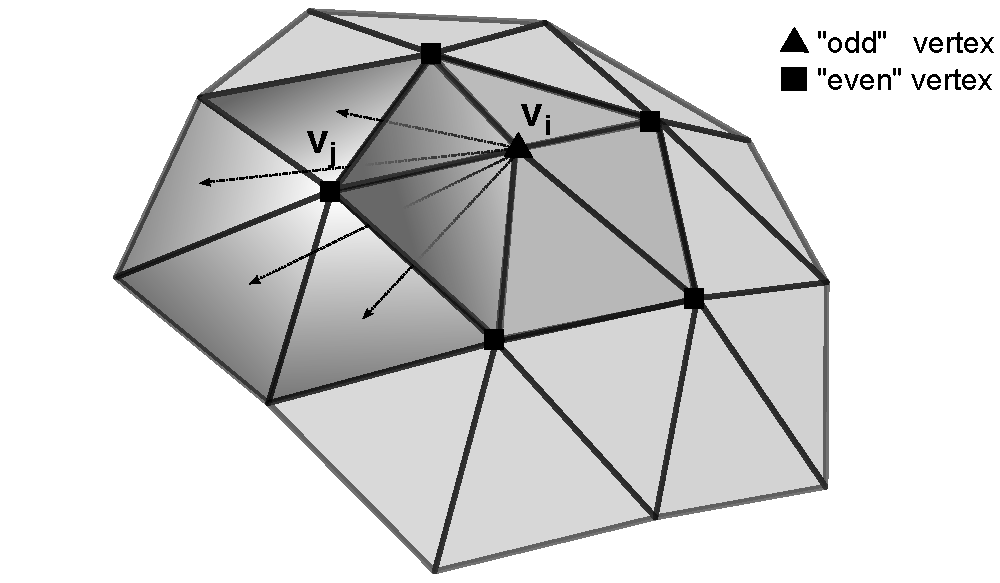
\includegraphics[width=.9\linewidth]{oneRingCost.pdf}
		%
		\caption{\label{fig_cds:oneRingCost}
			The cost of removing $\mathbf{v}_i$ with respect to its one-ring neighbours. Each $\mathbf{v}_j \in \mathcal{N}_v^1(\mathbf{v}_i)$ contributes
			the sum of distances from $\mathbf{v}_i$ to the support planes of each incident face at $\mathbf{v}_j$.}
	\end{figure}
	
	The purpose of computing the per-vertex cost values is to establish an importance-based ordering of this set. The greedy strategy we employ to label all vertices as either even or odd is summarized in algorithm \ref{alg_cds:labelling}. The labeling process is iterative and marks the vertices intuitively, according to their computed importance. During each iteration, the vertex having the lowest cost is extracted from the set of unmarked vertices. Its one-ring neighbors are then colored as even, while the extracted sample is marked as odd. The intuition behind the process reflects the goal of removing less relevant samples, from high redundancy areas.
	\begin{algorithm}[t]
		\begin{algorithmic}
			\STATE \texttt{INPUT}: the mesh $M=(V,E)$
			\STATE \texttt{OUTPUT}: an "odd-even" partitioning, $V = {V_o} \cup {V_e}$, coarse mesh topology $\tilde{M}=(V_e,\tilde{E})$
			\STATE \texttt{SORT}: $V^{*} = \mathtt{sort}(V)$ using $\mathtt{cost}(\mathbf{\bar{v}})$ as a key
			\STATE \texttt{ASSIGN}: $V_e = \emptyset, V_o = \emptyset$, $\tilde{E} = E$
			\WHILE { $ V^{*} \neq \emptyset $ }
			\STATE $\mathbf{v} = \arg\min\limits_{\mathbf{v} \in V^{*}}(\mathtt{cost}(\mathbf{v}))$
			\IF { \texttt{can\_triangulate}($\mathcal{N}_v^1(\mathbf{v}) \setminus \{\mathbf{v}\}$) }
			\FOR{$\mathbf{v}_i \in \mathcal{N}_v^1(\mathbf{v})$}
			\STATE $\tilde{E} = \tilde{E} \setminus \{\overline{\mathbf{v}, \mathbf{v}_i}\}$
			\ENDFOR
			\STATE $\tilde{E} = \tilde{E} \cup \mathtt{create\_edges}(\mathcal{N}_v^1(\mathbf{v}))$
			\STATE $V_o = V_o \cup \{\mathbf{v}\}$
			\STATE $V_e = V_e \cup \mathcal{N}_v^1(\mathbf{v})$
			\STATE $V^{*} = V^{*} \setminus \left( \{ \mathbf{v} \} \cup \mathcal{N}_v^1(\mathbf{v}) \right)$
			\ELSE
			\STATE $V_e = V_e \cup \{\mathbf{v}\}$
			\STATE $V^{*} = V^{*} \setminus \{ \mathbf{v} \}$
			\ENDIF
			\ENDWHILE
		\end{algorithmic}
		\caption{Vertex labeling and remeshing algorithm}
		\label{alg_cds:labelling}
	\end{algorithm}
	
	
	%\begin{figure}[htb]
	\begin{figure}[t]
		\centering 
		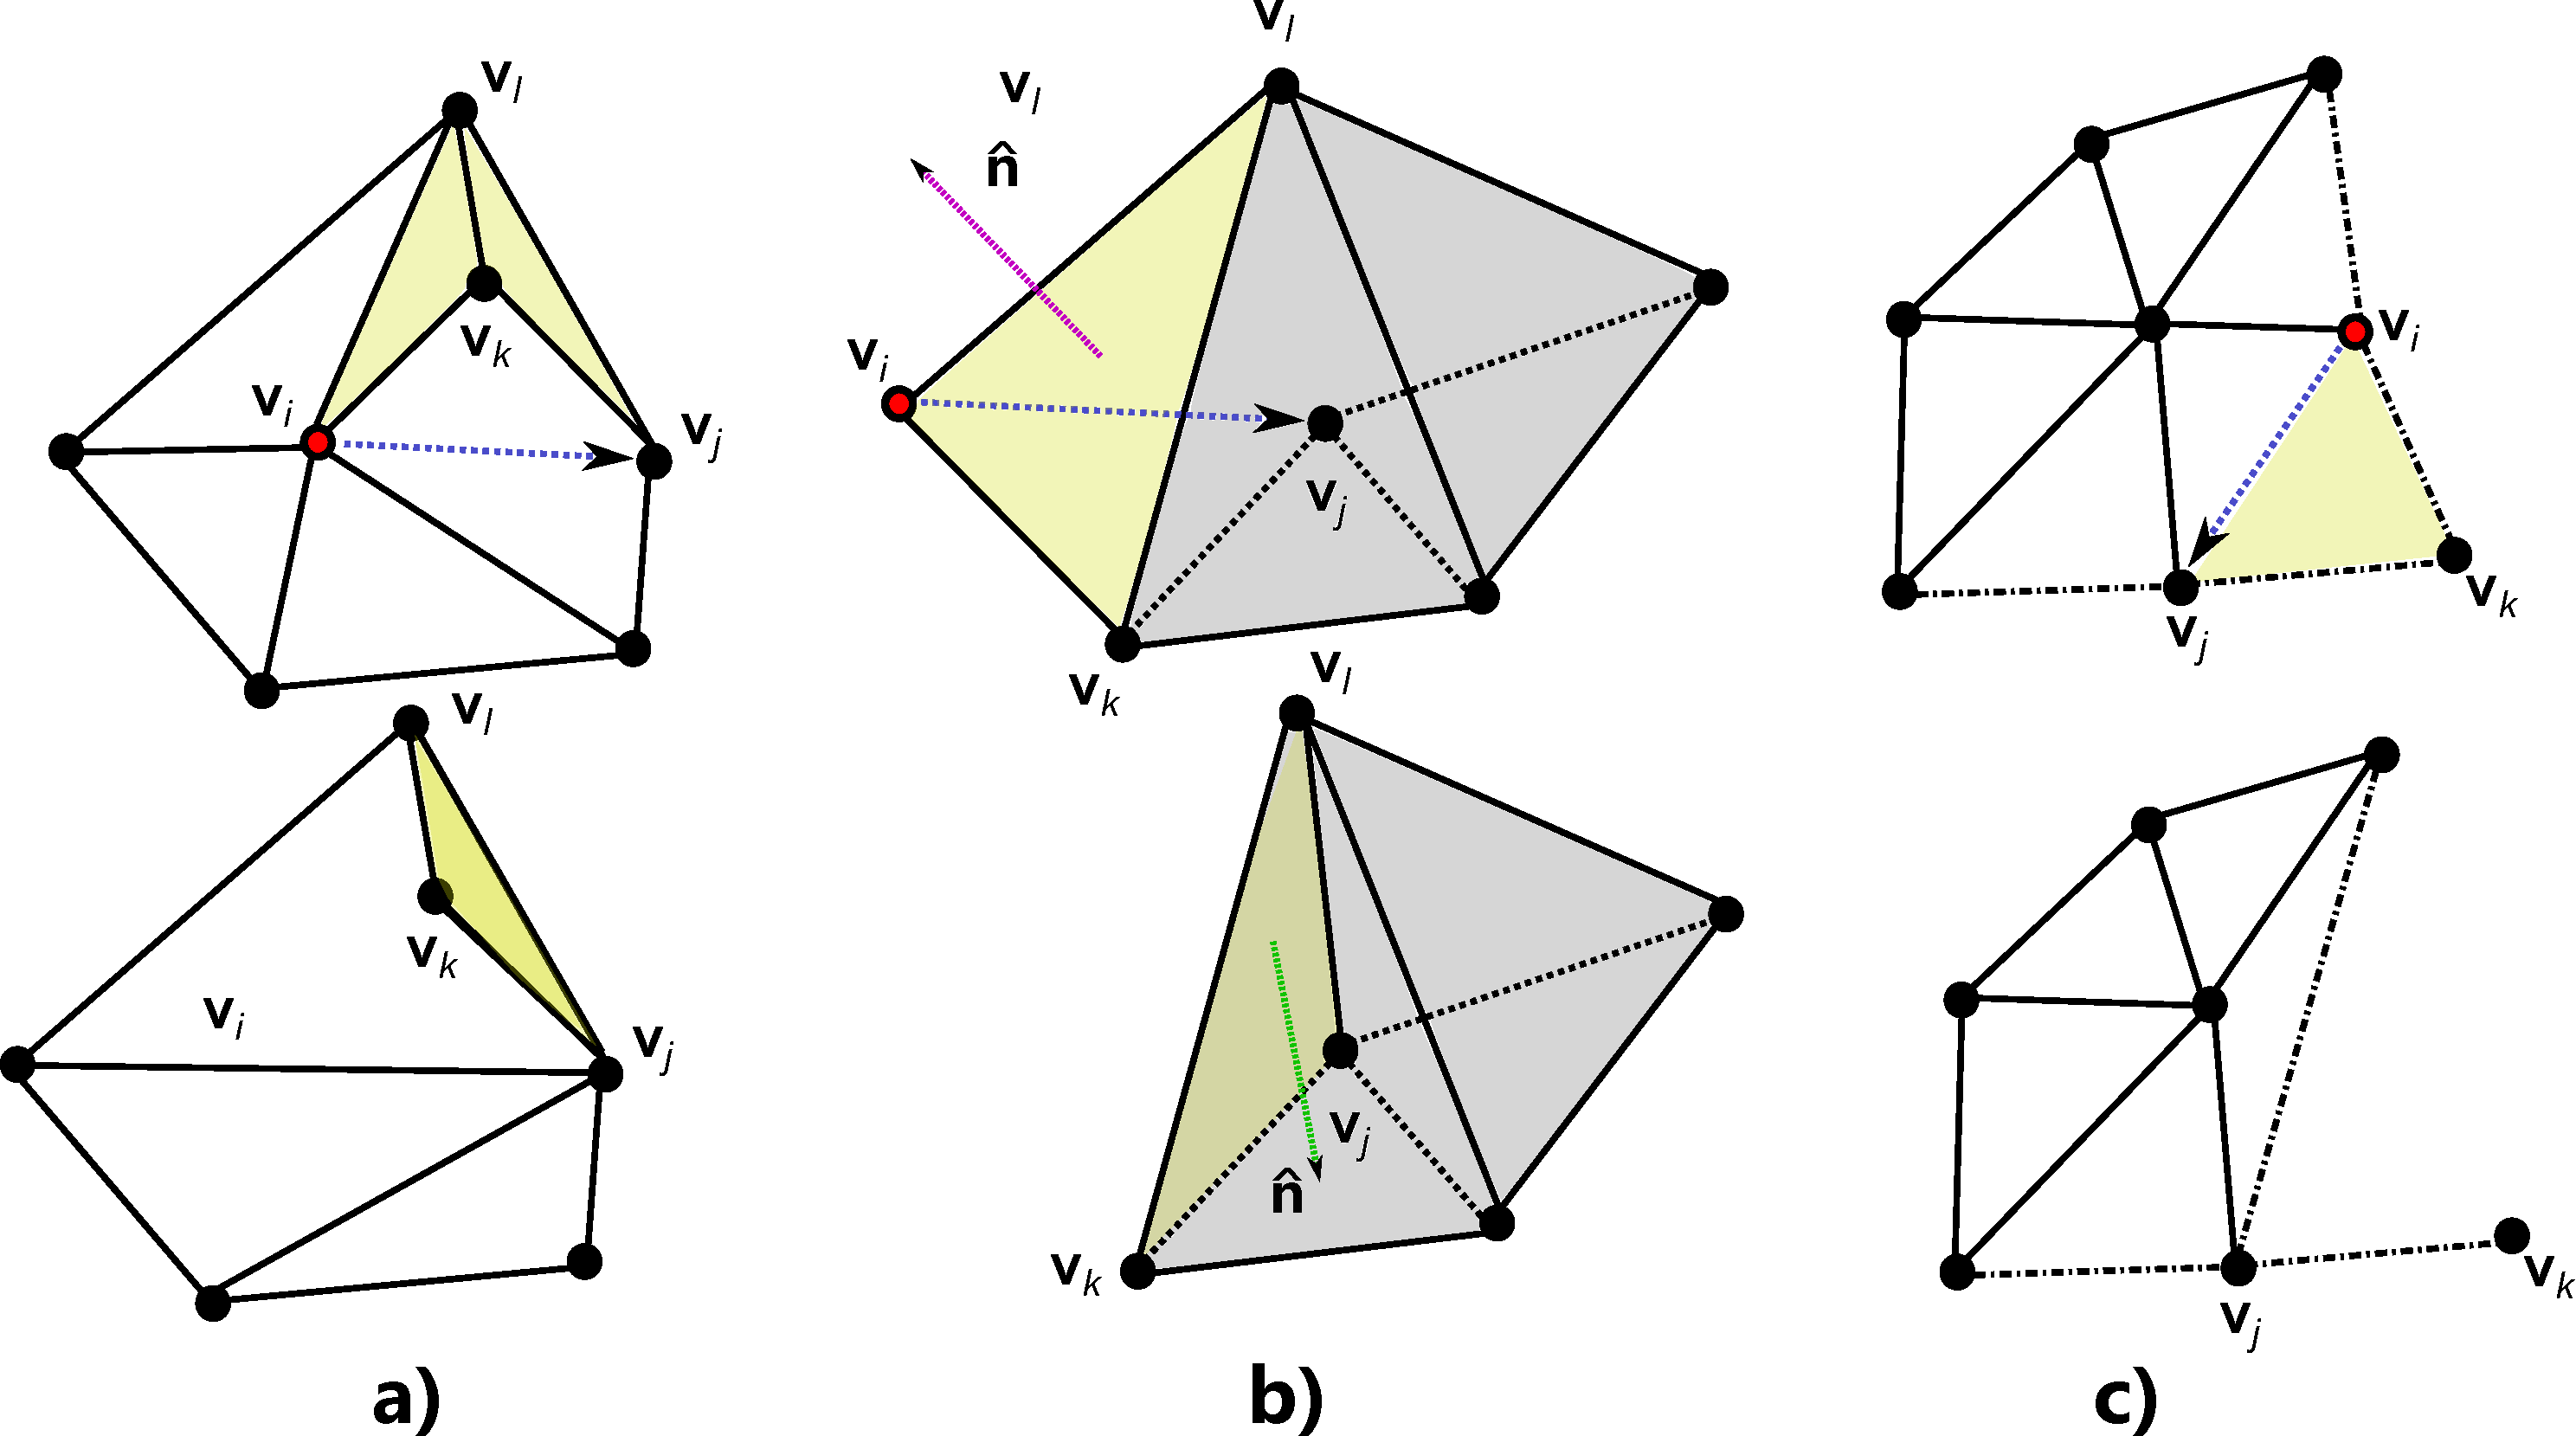
\includegraphics[width=.95\columnwidth]{forbidden_collapses.pdf} 
		\caption{Illegal collapse situations where the highlighted faces are involved in a breaching of one or several criteria of the $\mathtt{can\_triangulate}$ function from algorithm  \ref{alg_cds:labelling}. In case a), the collapse "welds" together two faces, back-to-back, introducing an edge common to more than two triangles. In situation b), the highlighted face is "flipped" since the normal unit vectors before and after the collapse point in opposite directions. "Cutting a corner" is the operation depicted in situation c), where the corner vertex is no longer adjacent to at least two edges.} 
		\label{fig_cds:forbidden_collapses} 
	\end{figure}
	
	Analyzing the vertex classification and remeshing performed by algorithm \ref{alg_cds:labelling}, we notice the constraint of marking the neighbors of a removed odd node as even. This is justified by the need to consistently separate the two vertex classes,  a practice also employed by \cite{Guskov1999}. Another key property of this algorithm is the partial graph connectivity alteration incurred by the removal of the odd samples. Together with these nodes, their adjacent edges are also removed. Whether or not the one-ring hole bounded by $\mathcal{N}_v^1(\mathbf{v})\setminus\{\mathbf{v}\}$ can be triangulated is also a key factor in deciding the label of $\mathbf{v}$. The $\mathtt{can\_triangulate}(\cdot)$ function is implemented as a set of geometrical and topological consistency criteria that must be satisfied by a valid triangulation. This problem has numerous solutions, one example being the \emph{splitting plane} method of \cite{Schroeder1992} known to produce more regular aspect ratio triangulations. It is possible for a vertex having the lowest importance score to produce invalid triangulations, and, in this case, the vertex is marked as even. In our implementation, the triangulation of the one-ring hole is easily performed using half-edge collapses. A valid edge is selected from the set of all edges adjacent to the removed odd vertex such that the quadric error measured using the $\mathbf{Q}(\mathbf{v}_e)$ matrix of its even endpoint is the smallest of all other collapsible pairs. We refer to a vertex pair to be collapsible if it is connected through an edge and if by translating the odd vertex over the even one the discrete manifold property of the mesh is not affected and no newly created triangular face is flipped with respect to its original normal vector (refer to figure \ref{fig_cds:forbidden_collapses} for several examples of illegal collapses). Additionally, to prevent boundary shrinkage, the odd boundary vertices cannot be translated over interior even ones. Boundary vertices can be part of a collapse if the edge connecting them is a boundary one as well. We also allow for merging an interior vertex with a boundary one when the collapse direction is from the interior towards the border.
	
	%In the remainder of this chapter, we adopt the $V_{o_l}$ and $V_{e_l}$ notations for denoting the odd vertex subset  and, respectively, the even vertex subset at level $l$.
	
	
	\subsubsection{Prediction filter construction}
	The goal of the prediction operation that follows the even-odd splitting is to compute estimates for the odd nodes of the graph from their even neighboring nodes. Intuitively, if the predicted values are closer to the actual odd samples, it is possible to recover a faithful representation of the entire graph by storing only a subset of the initial data. The resulting estimates are usually obtained by applying a low-pass filter to the even subset, while computing the difference between the estimates and the actual odd samples resembles the behavior of a high-pass filter. As a graph low-pass filter, we propose using a discrete Laplacian operator, given its smoothing and averaging effects. In many applications, Laplacian filters are also used for suppressing local irregularities (both features and noise). Thus, a similar effect could be achieved by removing the ensuing details.
	
	
	To understand how the prediction filter weights are computed, we recall the concept of a graph Laplacian operator. For a weighted graph, the Laplacian matrix is obtained as the difference between the weighted diagonal degree matrix, $\mathbf{D} = (d_{i,i}) = \sum_{j}{\omega_{i,j}}$, and the cost matrix, $\bm{\Omega} = (\omega_{i,j})$,
	where $\omega_{i,j}$ are the weights associated with the $(\mathbf{v}_i,\mathbf{v}_j)$ edges. Thus, if $\mathbf{L} = \mathbf{D} -  \bm{\Omega}$, the random-walk Laplacian operator is defined as
	\begin{equation}
	\mathcal{L}_{rw} = \mathbf{D}^{-1} \mathbf{L} =  \mathbf{I} - \mathbf{D}^{-1} \bm{\Omega}.
	\label{eq_cds:random_walk_laplacian}
	\end{equation}
	The geometric interpretation for the action this operation has on a mesh is a smoothing effect, also achievable through the use of a generalized umbrella operator.  An in-depth comparative discussion of various Laplacian discretizations  is offered by \cite{Wardetzky2007}. Concretely, the extraction of the difference vectors $\mathbf{w}_{l,V_{o_{l+1}}}$ from equation (\ref{eq_cds:prediction_difference_vectors}) is similar to a Laplacian smoothing where
	the difference between the smoothed vertex and its actual position is stored for later reference. For a single vertex, $\mathbf{v}_n \in V_{o_{l+1}}$, this equation can be rewritten as
	\begin{equation}
	\mathbf{w}_{l, \mathbf{v}_n} = \mathbf{s}_{l+1,\mathbf{v}_n} - \mathlarger{\mathlarger{\sum}}_{\mathbf{v}_m \in \mathcal{N}_v^1(\mathbf{v}_n)}{ p_{l, \mathbf{v}_n}(\mathbf{v}_m)  \mathbf{s}_{l+1,\mathbf{v}_m} },
	\label{eq_cds:prediction_vertex}
	\end{equation}
	where $p_{l, \mathbf{v}_n}(\mathbf{v}_m)$ is the prediction weight coefficient at level $l$ associated with vertex $\mathbf{v}_n$ and contributed by one of its even, one-ring neighbors, $\mathbf{v}_m$. Depending on the Laplacian discretization, several prediction weight choices are possible. In general, the prediction weights in equation (\ref{eq_cds:prediction_vertex}) are computed as
	\begin{equation}
	p_{l, \mathbf{v}_n}(\mathbf{v}_m) = \frac{ \omega_{n,m} } { \sum_{\mathbf{v}_k \in \mathcal{N}_v^1(\mathbf{v}_n)} { \omega_{n,k } }}.
	\label{eq_cds:prediction_weight}
	\end{equation}
	One of the more popular Laplacian design choices is the \emph{cotangent weights} Laplacian, computed as described by Meyer et al. \cite{Meyer2003}. Abdul Rahman et al. \cite{AbdulRahman2013} recommend this Laplacian as a prediction filter for the analysis of free-form surfaces with additional attributes. Although this filter is suitable for smoothing tasks, its weights depend strictly on the geometric information and not also on any additional attributes. A simple alternative for this operator, that introduces movements in the tangential plane of a vertex, is the Fujiwara or geometric Laplacian \cite{Fujiwara95}, with weights defined as
	\begin{equation}
	\omega_{i,j} = {l_{i,j}}^{-1}, 
	\label{eq_cds:fujiwara}
	\end{equation}
	where $l_{i,j}$ is the length of the $(\mathbf{v}_i,\mathbf{v}_j)$ edge. This operator is scale dependent and it preserves the distribution of triangle sizes. Several arguments support choosing this design are: its dependency on all geometry and range attributes, its smoothing effect being closer to the cotangent weight formulation than that of the umbrella operator, and the predicted point being shifted towards its closest neighbours, thus inherently providing a better approximation.
	
	An alternative to the Laplacian prediction filter is to employ a least squares fitting of the weights in order to minimize the approximation error. This approach, adopted in several works \cite{Wagner2005,Martinez2011}, proved to be numerically unstable when directly applied to terrain sets. To overcome this issue, Wagner et al. \cite{Wagner2005} did not include the boundary vertices in the downsampling process. In regions where the one-ring neighborhood does not have a convex  $(x,y)$ projection, negative weights can appear. Furthermore, the large magnitude of the weights may lead to numerical instability during the subsequent update stage. To counteract these effects, we propose  a non-negative least squares (NNLS) fitting of the weights in equation (\ref{eq_cds:prediction_vertex}), such that
	the magnitude of the $\mathbf{w}_{l, \mathbf{v}_n}$ vector is minimized. To achieve a similar Laplacian smoothing effect, the sum $\mathlarger{\sum}_{\mathbf{v}_m \in \mathcal{N}_v^1(\mathbf{v}_n)}{ p_{l, \mathbf{v}_n}(\mathbf{v}_m)}$ should be equal to $1$. This constraint can be directly added to the NNLS solver. By design, this modification improves the root mean square error throughout the hierarchical downsampling, as it will be later discussed in the results section. We note that positive and convex weights allow for the removal of odd boundary vertices. Nevertheless, computing these weights incurs a computational penalty, so we only recommend this choice for scenarios where minimizing the approximation error is crucial.
	
	In terms of storage complexity,  the Laplacian matrix is very sparse. As a consequence, the prediction matrix at level $l$, $\mathbf{P}_l$, is also sparse, each of its rows being populated with the weights used to predict the same odd vertex,
	$\mathbf{v}_n$, from its even neighbours.
	
	
	%%
	\subsubsection{Update filter construction}
	The heuristically guided lazy wavelet removal of details minimizes feature loss, but does not propagate detail loss to inferior levels. Wavelet transforms manage this problem by redistributing the extracted detail among the coarser scales.  This information is effectively contained in the difference vectors. Without compensating for these losses, the algorithm would mostly resemble incremental simplification. The update filter of the lifting scheme is responsible for distributing the lost details among the even vertices in a way that preserves an aggregate signal property such as signal average. We opt for this choice because it helps maintain both overall shape and decreases the approximation error, as we will later experimentally observe. 
	
	Because the prediction filter determines the amount of detail loss, the update filter should express a dependency on the prediction weights. In \cite{Martinez2011}, the authors suggest the following expression for the update filter vectors:
	\begin{equation}
	\mathbf{u}_{l, \mathbf{v}_{u}} = \frac{0.5}{ \sum\limits_{\mathbf{v}_{p,i} \in \mathcal{N}_v^1(\mathbf{v}_u) \cap V_{o_{l+1}}} {  p_{l, \mathbf{v}_{p,i} } } } \left[ p_{l, \mathbf{v}_{p,1} }, p_{l, \mathbf{v}_{p,2} }, \ldots , p_{l, \mathbf{v}_{p,k} }\right],
	\label{eq_cds:smoothing_update_weights}
	\end{equation}
	where $\mathbf{v}_u$ represents an even vertex, $\mathbf{v}_{p,i}$ denotes an odd one-ring neighbour of this vertex, and $p_{l,\mathbf{v}_{p,i}} \equiv p_{l,\mathbf{v}_{p,i}}(\mathbf{v}_u)$ is the prediction weight $\mathbf{v}_u$ contributed in estimating its $\mathbf{v}_{p,i}$ odd neighbour.
	By using this design, there is no guarantee the signal average will be preserved, unless applied to unweighted graphs, hence when using the umbrella operator Laplacian.
	
	Abdul-Rahman et al. \cite{AbdulRahman2013} proposed a similar approach where the update filter construction aims to directly preserve the average value of the one-ring neighborhood of an odd vertex before and after its removal. Using the same update vector for all even neighbours, the following equation ensues:
	\begin{eqnarray}
	\frac{1}{ N + 1} \left( \mathbf{w}_{l, \mathbf{v}_n} + \sum\limits_{\mathbf{v}_m \in \mathcal{N}_v^1(\mathbf{v}_n) } { (  p_{l, \mathbf{v}_n}(\mathbf{v}_m) + 1 ) \mathbf{s}_{l+1, \mathbf{v}_m} } \right) = \\ \frac{1}{N} \sum\limits_{\mathbf{v}_m \in \mathcal{N}_v^1(\mathbf{v}_n) } { (  \mathbf{s}_{l+1, \mathbf{v}_m} + \mathbf{u}_{l,\mathbf{v}_m} ) } ,
	\label{eq_cds:one_ring_average}
	\end{eqnarray}
	with $N = | \mathcal{N}_v^1(\mathbf{v}_n) |$, and the update vectors $\mathbf{u}_{l,\mathbf{v}_i} = \mathbf{u}_{l,\mathbf{v}_j} = \mathbf{u}_{\mathcal{N}_v^1(\mathbf{v}_n)} $ for any $\mathbf{v}_i, \mathbf{v}_j \in \mathcal{N}_v^1(\mathbf{v}_n)$. Thus, the uniform update vector is determined as
	\begin{equation}
	\mathbf{ u}_{\mathcal{N}_v^1(\mathbf{v}_n)} = \frac{1}{N + 1} \mathbf{w}_{l, \mathbf{v}_n}  + \sum\limits_{\mathbf{v}_m \in \mathcal{N}_v^1(\mathbf{v}_n) } { \frac{ N  p_{l, \mathbf{v}_n}(\mathbf{v}_m) - 1 }{N (N +1 ) } \mathbf{s}_{l+1, \mathbf{v}_m} }.
	\label{eq_cds:update_vector_one_ring}
	\end{equation}
	In case the prediction filter weights correspond to the umbrella operator type of Laplacian, the second term in equation (\ref{eq_cds:update_vector_one_ring}) vanishes. Generally, this design requires storing update weights for both difference vectors and even nodes from the previous level, thus becoming a more memory consuming approach.
	By aiming to directly preserve the one-ring average of the scaling coefficients, it becomes more difficult to find update weights that depend only on the difference vectors. This is due to the fact that determining such weights implies solving a sparse system involving all scaling coefficients. In the multi-variate scenario, this system becomes overdetermined and an exact solution may not exist. In this situation, an approximate solution must be searched for. In its terms, this is a process more complex than the entire lifting pipeline.
	
	In \cite{Cioaca2016} we also considered the solution proposed by Jansen et al. \cite{Jansen2001}. In principle, it also exploits the average preserving requirement. This prerequisite provides a mathematical constraint that can be expressed in terms of the integrals of the scaling functions, as described for the one-dimensional context discussion. Let $\varsigma_{l,\mathbf{v}_u}$ be the integral of the scaling function $\phi_{l, \mathbf{v}_u}$ (i.e. an element 
	of $\Phi_{l,V_{e_{l+1}}}$ corresponding to the vertex $\mathbf{v}_u \in E_l$). Rewriting equation (\ref{eq_cds:int_scaling}), we obtain
	\begin{equation}
	\varsigma_{l,\mathbf{v}_u} = \varsigma_{l+1, \mathbf{v}_u} + \mathlarger{\mathlarger{\sum}}_{\mathbf{v}_k \in \mathcal{N}_v^1(\mathbf{v}_u) \cap V_{o_{l+1}}} { p_{l,\mathbf{v}_k}(\mathbf{v}_u)
		\varsigma_{l+1, \mathbf{v}_k}} .
	\label{eq_cds:integral_update}
	\end{equation}
	The wavelet biorthogonality condition requires for each wavelet function to have zero integral. In consequence, when integrating equation (\ref{eq_cds:update_functions}) the left hand side
	term vanishes, i.e.,
	\begin{equation}
	0 = \varsigma_{l+1,V_{o_{l+1}}} - \mathbf{U}_l \varsigma_{l,V_{e_l}}.
	\label{eq_cds:integral_wavelet}
	\end{equation} 
	Further rewriting equation (\ref{eq_cds:integral_odd_node}) for each predicted vertex, $\mathbf{v}_p \in V_{o_{l+1}}$, leads to
	\begin{equation}
	\varsigma_{l+1,\mathbf{v}_p} = \mathbf{u}_{l,\mathbf{v}_p}^\intercal \varsigma_{l, \mathcal{N}_v^1(\mathbf{v}_p)},
	\label{eq_cds:scaling_function_integral}
	\end{equation}
	where $\mathbf{u}_{l,\mathbf{v}_p}$ is the vector containing the update weights this vertex contributes with for each of its one-ring, even vertices. Finding $\mathbf{u}_{l,\mathbf{v}_p}$
	requires solving an overdetermined equation of the form $\alpha = \mathbf{u ^\intercal v}$, where $\mathbf{u}$ is the unknown vector. From all possible solutions, both Jansen et al. \cite{Jansen2001} and Wagner et al. \cite{Wagner2005} choose the minimum update norm solution due to its stabilizing effect. This translates into setting $\mathbf{u} = \frac{\alpha \mathbf{v}}{\| \mathbf{v} \|^2}$. 
	Finally, equation (\ref{eq_cds:update_column_vector}), which gives the expression of the update vector of coefficients for $\mathbf{v}_p$, becomes
	\begin{equation}
	\mathbf{u}_{l,\mathbf{v}_p} = \frac{\varsigma_{l+1,\mathbf{v}_p}}{\sum_{\mathbf{v}_k \in \mathcal{N}_v^1(\mathbf{v}_p)} \varsigma_{l,\mathbf{v}_k}^2}
	\varsigma_{l, \mathcal{N}_v^1(\mathbf{v}_p)} .
	\label{eq_cds:update_coefficient_vector}
	\end{equation}
	With these results, the update equation (\ref{eq_cds:update_even_coefficients}) of an even scaling coefficient for a vertex $\mathbf{v}_u$ is written as
	\begin{equation}
	\mathbf{s}_{l, \mathbf{v}_u} = \mathbf{s}_{l+1,\mathbf{v}_u} + \mathlarger{\mathlarger{\sum}}_{\mathbf{v}_n \in \mathcal{N}_v^1(\mathbf{v}_u) \cap V_{o_{l+1}}} { u_{l, \mathbf{v}_u}(\mathbf{v}_n) \mathbf{w}_{l,\mathbf{v}_n} }.
	\label{eq_cds:update_even_scaling_coefficient}
	\end{equation}
	The choice of the scaling functions does not affect the so far described transform. Since the initial integrals $\varsigma_{l+1,E_{l+1}}$ need to be computed, one option is to assume a
	choice of the scaling functions such that these integrals are all equal to $1$.
	
	
	%--------------------------
	Given the fact that a terrain mesh has sparse connectivity, the filter matrices are also sparse. Each odd node is surrounded 
	by even nodes, ensuring a 25\% average reduction factor for each decimation stage. Asymptotically, almost 80\% of the initial edge density will still be required to store the 
	filter matrices. Nevertheless, the information is still very sparse and lends itself for specific algebraic manipulations after the cascaded analysis stages. 
	
	\subsection{Algorithm overview}
	The lifting scheme flow depicted in figure \ref{fig_cds:lifting_diagram} is at the core of the iterative downsampling process, illustrated in figure \ref{fig_cds:overview_downsampling} and summarized in algorithm \ref{alg_cds:downsampling}. In overview, we can identify three main stages: the cost computation, the labeling or \emph{lazy wavelet} decomposition and the analysis itself. Together, these stages resemble the structure of a classical filter bank.
	
	\begin{algorithm}[t]
		\begin{algorithmic}
			\STATE \texttt{INPUT}: a $d$-dimensional point cloud consisting of vertex-attribute pairs.
			\STATE \texttt{OUTPUT}: the lowest resolution vertex set, $\mathbf{s}_{0, V_0}$, the chain of prediction and update matrices, $(\mathbf{P}_l)_l$ and $(\mathbf{U}_l)_l$, and
			the string of difference vectors, $(\mathbf{w}_{l,V_{o_{l+1}}})_l$, where $l$ ranges from $0$ to the total number of refinement levels, $L$.
			
			\STATE \texttt{TRIANGULATE:} the input set, $V_L$.
			
			\FOR {l := L - 1 \textbf{downto} 0 }
			
			\STATE \texttt{COMPUTE:} the removal cost of each vertex using algorithm \ref{alg_cds:thin_plate_energy}
			\STATE \texttt{PARTITION:} the vertex set $V_{l+1} = V_{e_{l+1}} \cup V_{o_{l+1}}$ using algorithm \ref{alg_cds:labelling}.
			
			\STATE \texttt{COMPUTE:} $\mathbf{w}_{l,V_{o_{l+1}}}$ and $\mathbf{s}_{l,V_{e_{l}}}$ from $\mathbf{s}_{l+1,V_{e_{l+1}}}$ using equations (\ref{eq_cds:prediction_difference_vectors}) 
			and (\ref{eq_cds:update_even_coefficients})
			\STATE \texttt{STORE:} $\mathbf{P}_l$, $\mathbf{U}_l$ and $\mathbf{w}_{l,V_{o_{l+1}}}$
			\ENDFOR
			\STATE \texttt{STORE:}  $\mathbf{s}_{0,V_0}$
		\end{algorithmic}
		\caption{Downsampling algorithm}
		\label{alg_cds:downsampling}
	\end{algorithm}
	
	\begin{figure}[htb]
		\centering
		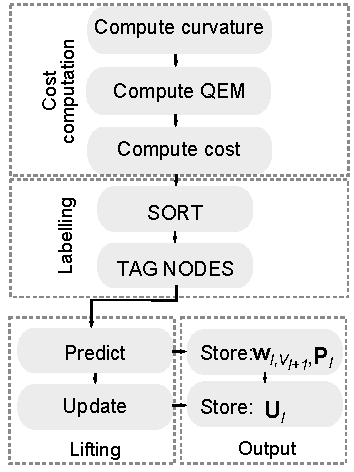
\includegraphics[width=.7\linewidth]{overview_downsampling.pdf}
		%
		\caption{\label{fig_cds:overview_downsampling}
			An overview of our hybrid algorithm for downsampling an input set.}
	\end{figure}
	
	This algorithm has $O(N \log N)$ complexity (where $N$ is the total number of vertices). This higher complexity is due to the 
	nodes being sorted according to their removal cost. While an $O(N)$ complexity is achievable, the salient
	features will not be preserved as faithfully (see figure \ref{fig_cds:sharpFeatures}). The initial triangulation can be performed only once, during the pre-processing stage. During the downsampling steps, the one-rings of the odd vertices can be re-triangulated on the fly, keeping a consistent manifold connectivity. 
	
	The spatial complexity of this method is linear with respect to the size of the input data set. More precisely, the lowest resolution data and the difference vectors require the same
	amount of storage as the initial point cloud. Empirically, the triangulated meshes will not be far from semi-regular, thus the prediction weights will require $6N$ scalars in total. 
	For the update weights, sparse structures corresponding to even vertices being surrounded by 3 odd vertices on average have to be stored. Assuming a decimation rate of $25\%$, the
	spatial requirements for storing the update weights asymptotically approach $15N$.
	%%
	%%
	
	\subsubsection{Quadric error matrix update procedure}
	The quadric error metric matrix fusion of collapsed vertex pairs is a property that we adapt locally, in the odd vertex neighborhood. We achieve this by distributing the matrix corresponding to an odd sample, $\mathbf{Q}({\mathbf{v}_{o_{j+1}}})$, among its even neighbors. Thus, each even matrix is updated by
	\begin{equation}
	\mathbf{Q}({\mathbf{v}_{e_j}}) = \mathbf{Q}({\mathbf{v}_{e_{j+1}}}) + \sum\limits_{\mathbf{v}_{o_{j+1}} \in \mathcal{N}^1_v(\mathbf{v}_{e_{j+1}}) \cap V_{o_{j+1}} } { \rho{j, \mathbf{v}_{e_{j+1}} }(  \mathbf{v}_{o_{j+1}}) \mathbf{Q}({ \mathbf{v}_{o_{j+1}}} )} ,
	\label{eq_cds:qem_update}
	\end{equation}
	where $\rho{j, \mathbf{v}_{e_{j+1}} }(  \mathbf{v}_{o_{j+1}})$ is the redistribution weight describing the influence of $ \mathbf{v}_{o_{j+1}}$ on its even neighbor, $\mathbf{v}_{e_{j+1}}$. We propose using the same weights that the prediction filter relies on estimating the lost information, i.e.,
	\begin{equation}
	\rho{j, \mathbf{v}_{e_{j+1}} }(  \mathbf{v}_{o_{j+1}}) =  \frac{p_{j, \mathbf{v}_{o_{j+1}} }(  \mathbf{v}_{e_{j+1}})}
	{ \sum_{\mathbf{v}_{u_{j+1}} \in \mathcal{N}^1_v(  \mathbf{v}_{o_{j+1}}) } { p_{j, \mathbf{v}_{o_{j+1}} }(  \mathbf{v}_{u_{j+1}}) }}.
	\label{eq_cds:qem_weights}
	\end{equation} 
	This choice is natural since the even vertex that contributes more to the prediction of an odd neighbor receives a larger fraction of its quadric error matrix. We justify this to be a more natural choice given that most prediction weights automatically encode a node similarity magnitude.
	Other quadric error matrix redistribution weights choices  and strategies are possible and were analyzed in \cite{Cioaca2015} and \cite{Cioaca2016UPB}. Experimentally, the choice of weights presented through equation (\ref{eq_cds:qem_weights}) was determined to achieve, on average, slightly more accurate approximations than the alternatives presented in \cite{Cioaca2016UPB}.
	
	
	\section{Numerical and visual experiments}
	
	We assessed the validity and efficiency of our method through a series of experiments involving three different LiDAR sets. The first model is a scan fragment of the Great Smoky Mountains (available through the {\url{www.opentopography.org/}} portal) with a density of approximately 2.23 points per square meter and a size of 280,000 points (figure \ref{fig_cds:smokey_lod_rmse}).  The second set is larger and much denser at approximately 20 points per square meter and a count of 9 million (figure \ref{fig_cds:fundata_lod_rmse}). 
	The third set is larger but less denser, consisting of 11.5 million points, at a density of 5 points per square meter (figure \ref{fig_cds:iezer_lod_rmse}). These larger and denser LiDAR samples were acquired through custom aerial scans conducted over two regions of the Romanian Carpathians. All terrain samples contain both geometry (point coordinates) and attribute information (i.e., vegetation type, as a scalar between 0 and 20, and height above ground, as a scalar between 0 and 30).
	All coordinates are translated and scaled to fit within a zero-centered unit bounding box dividing them by their range width. This way we significantly alleviate the effect of the diverse scales
	on the final outcome. However, the attributes could be scaled
	differently if one desires to diminish or enhance their contribution.
	
	\subsection{Root mean squared error measurements}
	
	As a measure of quality and accuracy, we have chosen the root mean square error (RMSE). Although other error measuring mechanisms exist, the RMSE or $L_2$ norm is one of the simplest and most efficient indicators of shape and attribute quality (see \cite{Payan2006} for a more in-depth discussion of the properties and applications of this error). In our case, the RMSE computation concerns both geometry and attribute vertex coordinates, except for the artificially added bending energy. Thus, if $\mathbf{s}_{l,\mathbf{v}_i}$ is the scaling coefficient at level $l$ of a node $\mathbf{v}_i$, and $\mathbf{s}_{L,\mathbf{v}_i}$ is the corresponding coefficient in the initial input set, the RMSE is evaluated as
	
	\begin{equation}
	\mathtt{RMSE}_l = \sqrt{\sum_{\mathbf{v}_i \in E_l}{ \| \mathbf{s}_{L,\mathbf{v}_i} - \mathbf{s}_{l,\mathbf{v}_i } \|^2 } } .
	\label{eq_cds:RMSE}
	\end{equation}
	
	
	For the multiresolution representation experiments, we have also considered several prediction and update filter designs. In this respect, we labeled the result sets according to the type of prediction and update filters as follows:
	\begin{itemize}
		\item{\emph{prediction filters}}: uniform weights obtained by using the unweighted graph Laplacian (\textbf{UG}), used in several works such as those of Martinez and Ortega \cite{Martinez2011} and of \cite{AbdulRahman2013}, the cotangent Laplacian weights (\textbf{CL}), also used Abdul-Rahman et al., the Fujiwara or geometric Laplacian (\textbf{GL}), which is our proposal for a Laplacian design for multi-variate data and a constrained  non-negative least squares weights design (abbreviated as \textbf{NNLS}), which we propose in order to minimize the detail vector norms.
		\item{\emph{update filters}}: the filter design proposed by Martinez and Ortega \cite{Martinez2011} compensates for the detail loss incurred by the removal of the "odd" vertices, but it does not preserve the graph signal average for weighted graphs, unless all weights are uniform. On the other hand, the design used in \cite{Jansen2001,Wagner2005}, achieves this goal while minimizing the norm of the update coefficient vectors. To distinguish between the first option and the minimum norm update weights, we have added the \textbf{MN} suffix to the prediction filter abbreviation. The third and final design option, proposed in \cite{AbdulRahman2013}, preserves the local, one-ring mean of the data samples  and is abbreviated as \textbf{ORMP}.
	\end{itemize}
	
	\begin{figure*}[!htbp]
		\centering
		% the following command controls the width of the embedded PS file
		% (relative to the width of the current column)
		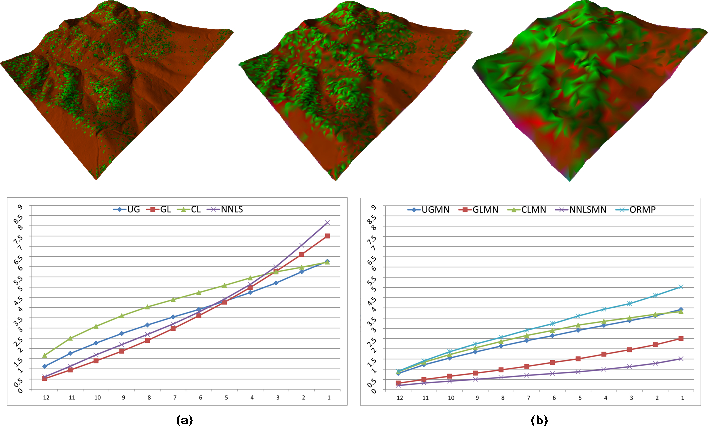
\includegraphics{smokey_lod_rmse.pdf}
		
		\caption{\label{fig_cds:smokey_lod_rmse}%
			Smoky Mountains fragment. Top row, left to right: shape and attribute evolution at levels 0, 12 and 24 using the \textbf{UG} filters. Bottom row: comparative charts for the RMSE evolution across 12 analysis sequences. }
	\end{figure*}
	
	\begin{figure*}[!htbp]
		\centering
		% the following command controls the width of the embedded PS file
		% (relative to the width of the current column)
		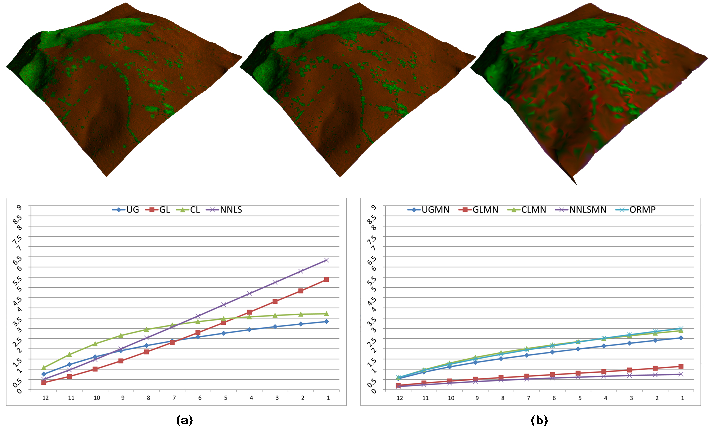
\includegraphics{fundata_lod_rmse.pdf}
		
		\caption{\label{fig_cds:fundata_lod_rmse}%
			High-density Carpathian Mountains fragment.  Top row, left to right: shape and attribute evolution at levels 0, 12 and 24 the \textbf{UG} filters. Bottom row: comparative charts for the RMSE evolution across 12 analysis sequences. }
	\end{figure*}
	
	\begin{figure*}[!htbp]
		\centering
		% the following command controls the width of the embedded PS file
		% (relative to the width of the current column)
		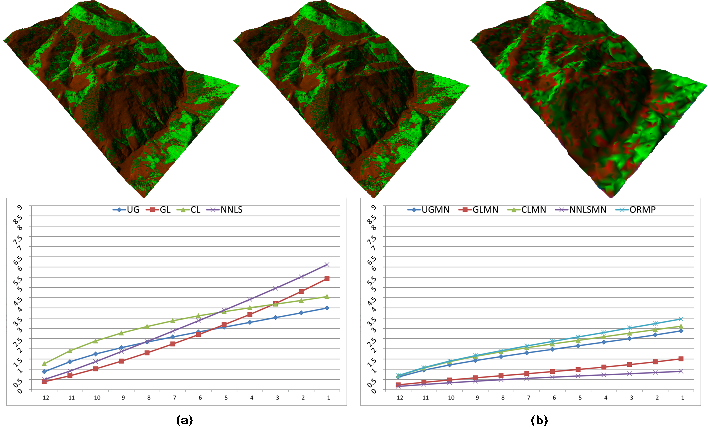
\includegraphics{iezer_lod_rmse.pdf}
		
		\caption{\label{fig_cds:iezer_lod_rmse}%
			Low-density Carpathian Mountains fragment.  Top row, left to right: shape and attribute evolution at levels 0, 12 and 24 the \textbf{UG} filters. Bottom row: comparative charts for the RMSE evolution across 12 analysis sequences. }
	\end{figure*}
	
	\subsection{Feature selectivity and robustness to noise}
	For a proof of concept, we subjected the Smoky Mountains terrain fragment to a sequence of 8 analysis steps. The same set was again analyzed using the lazy-wavelet partitioning strategy employed in \cite{Wagner2005, Martinez2011}. Without our proposed feature preservation
	heuristic, the lowest resolution representation will lose a bigger fraction of the sharp features, as depicted in figure \ref{fig_cds:sharpFeatures}.
	
	\begin{figure}[!htbp]
		\centering
		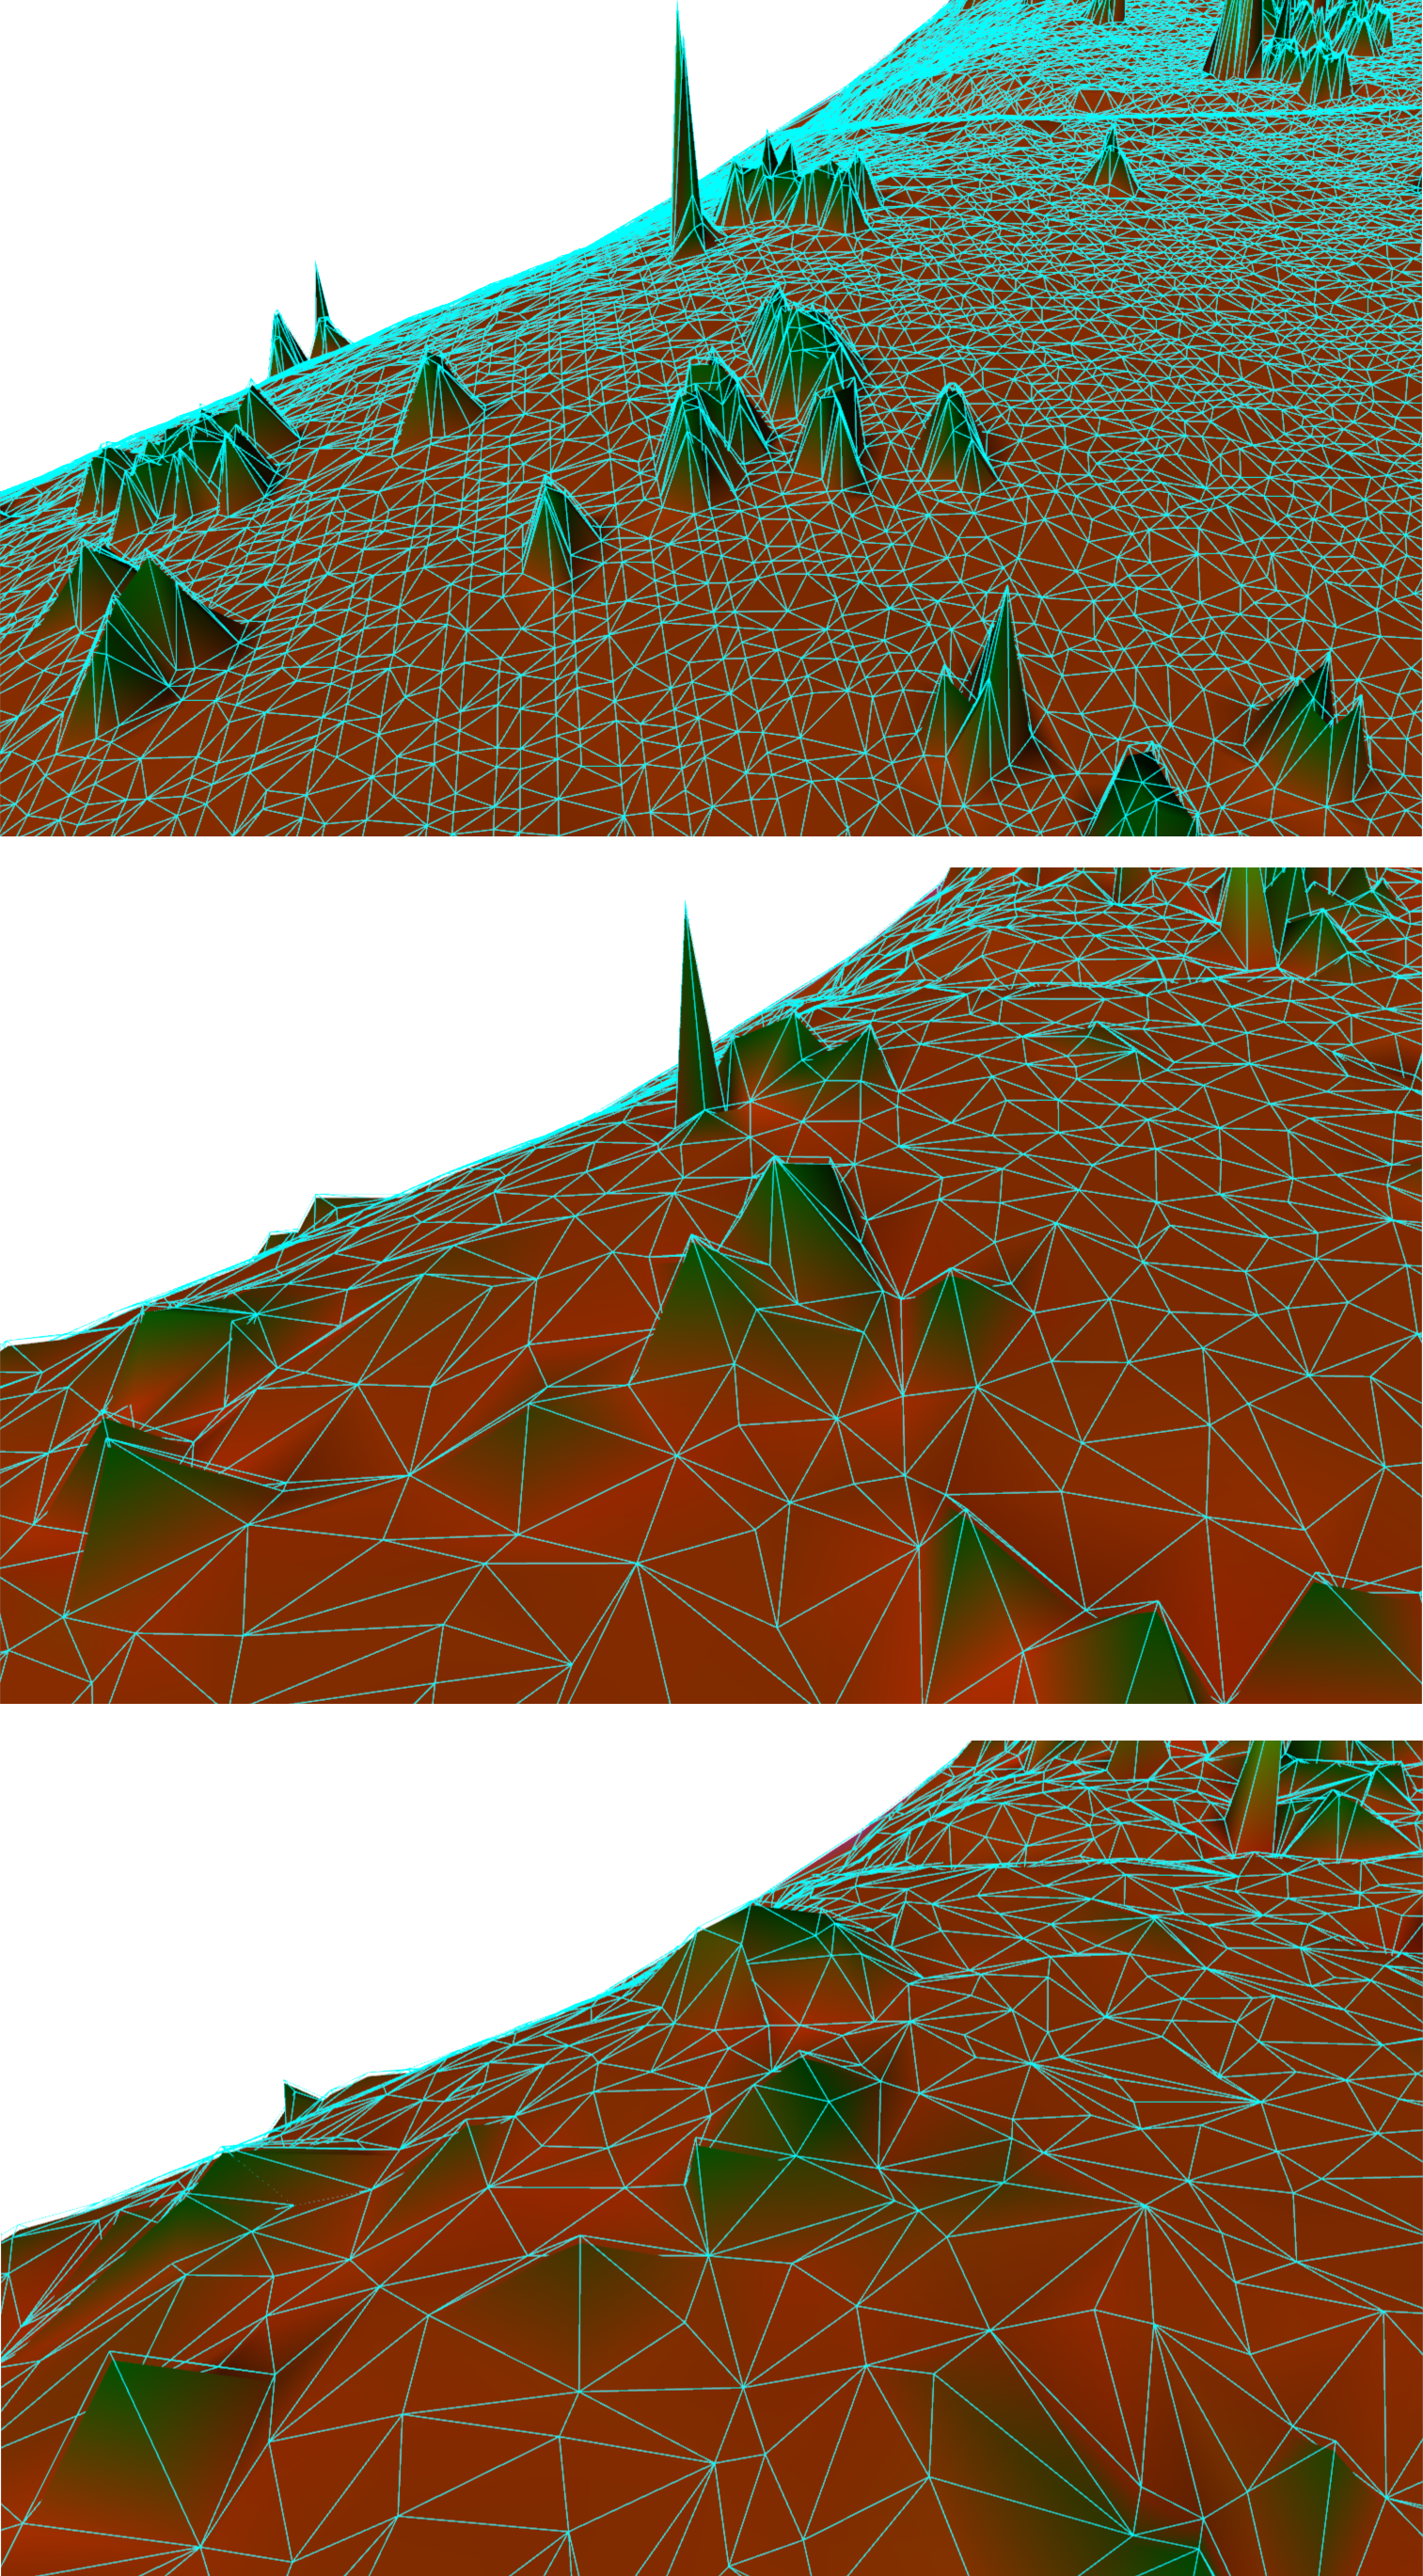
\includegraphics[width=0.75\linewidth]{QEMvsNO.png}
		%
		\caption{\label{fig_cds:sharpFeatures}
			Preservation of salient features after 8 analysis steps. Top image: high-density, high-detail input (1.6M faces), middle image (160K triangles): the combined QEM and thin plate energy cost, bottom image (158K triangles): the graph colouring strategy used in \cite{Wagner2005} and \cite{Martinez2011}. }
	\end{figure}
	
	
	Computing the discrete curvatures using the method of \cite{Meyer2003} is recommended for meshes with low to no noise. In \cite{Cioaca2016} and \cite{Cioaca2016CEAI}, we have experimentally shown that the proposed heuristic partitioning of the data points into odd and even categories is robust to noise.
	
	\subsection{Vertex frequency analysis interpretation}
	\begin{figure}[!htbp]
		\centering
		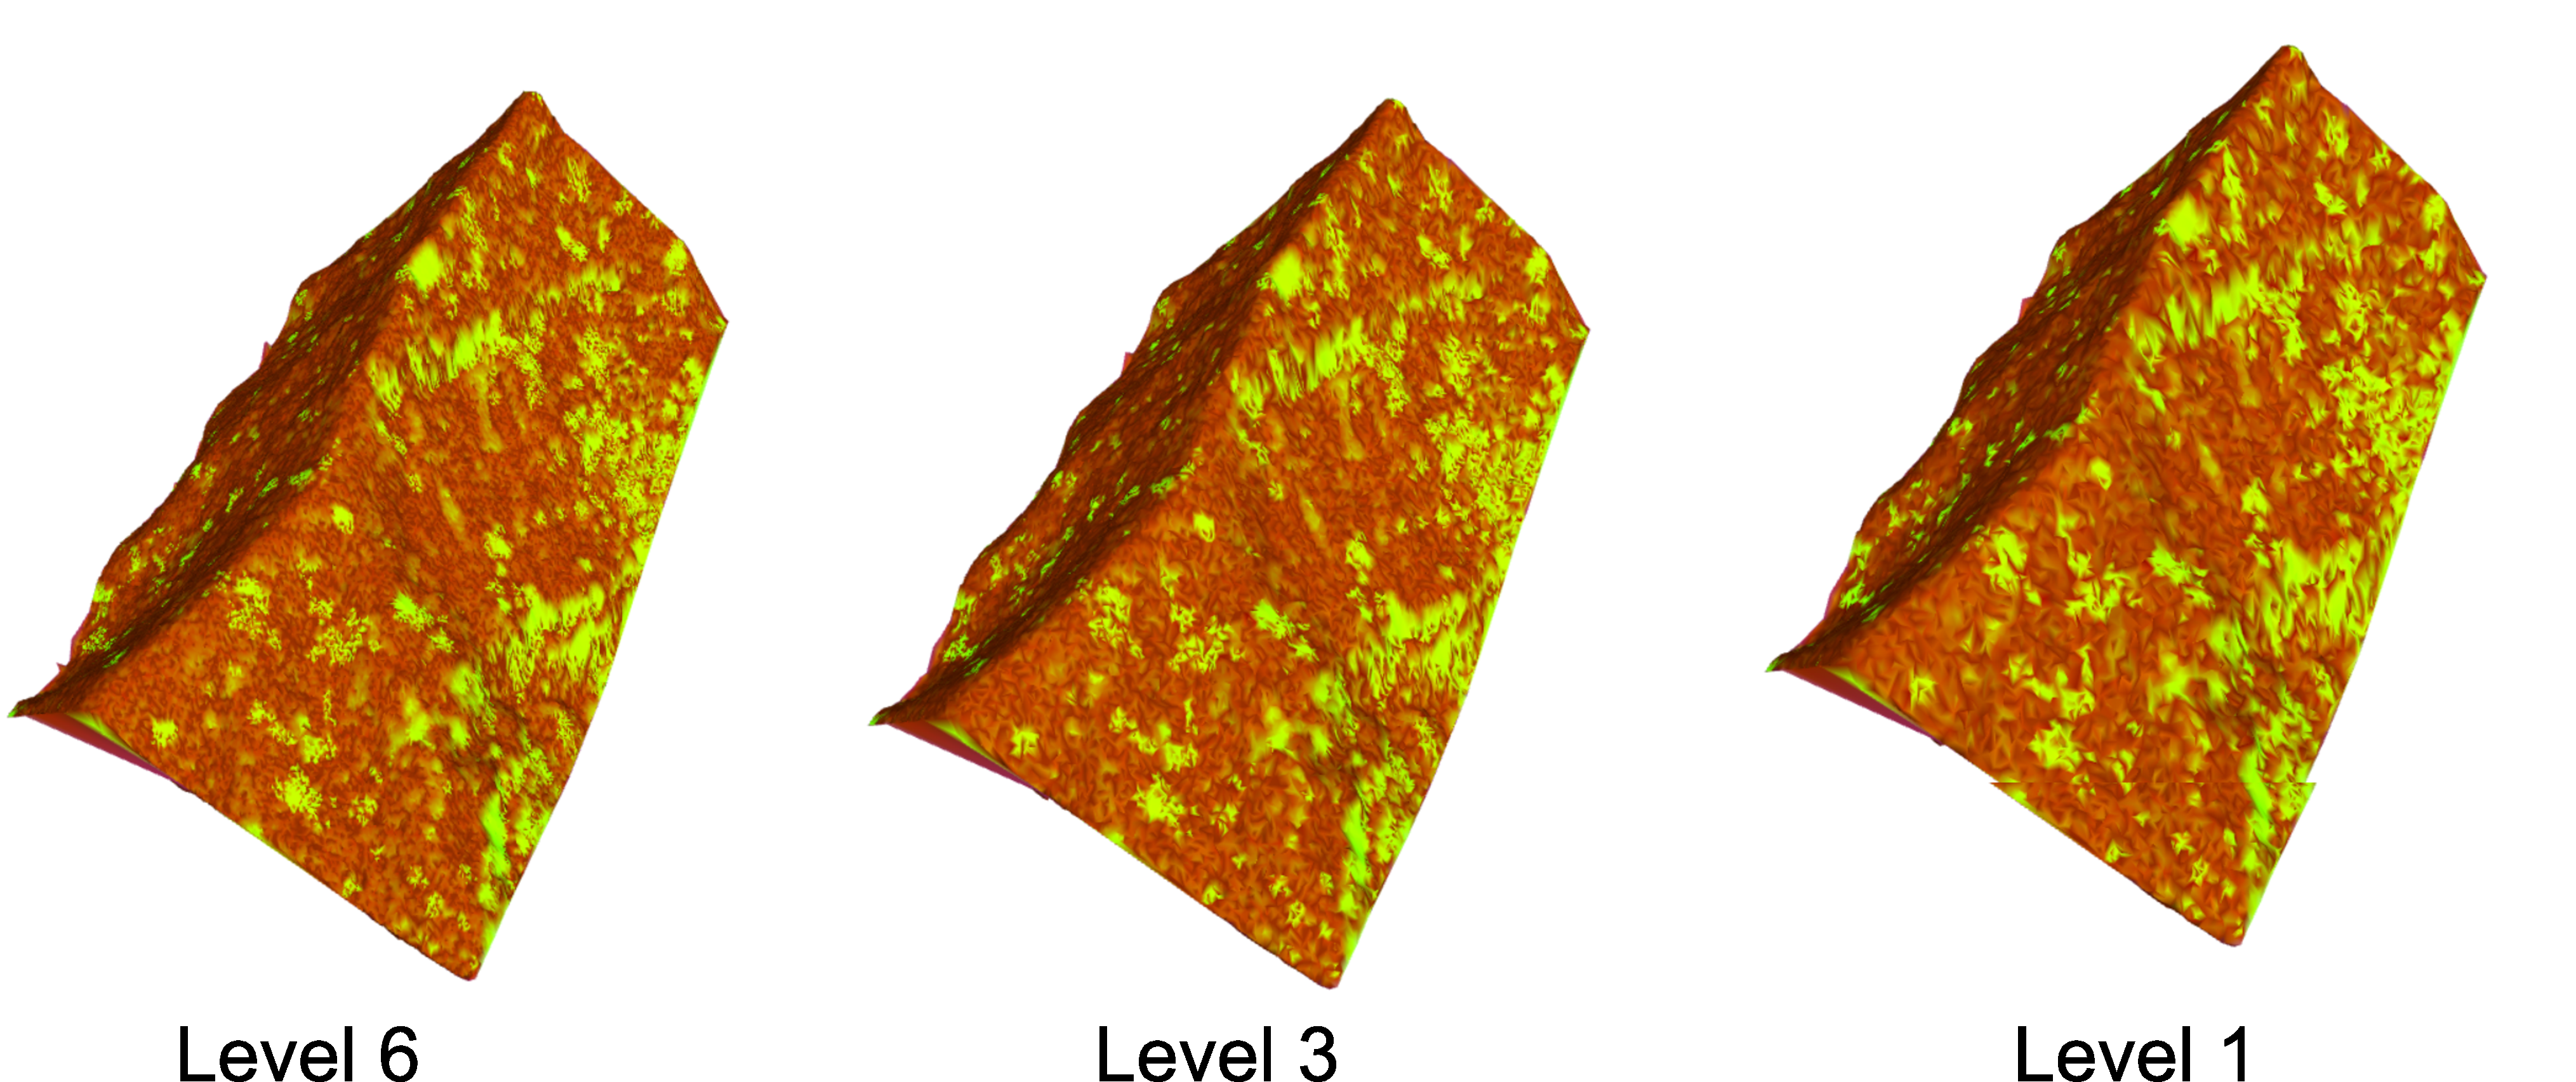
\includegraphics[width=1\linewidth]{Kauai5.pdf}
		%
		\caption{\label{fig_cds:Kauai}
			Kauai Mountain fragment consisting of 79,000 point samples. Represented are level 6, 3 and 1 corresponding to the initial set, the middle resolution and the lowest resolution in a cascade of 5 analysis passes. }
	\end{figure}
	
	Vertex frequency analysis is a more recently developed subfield of Graph Signal Processing. This subfield discusses solutions for a graph equivalent of time and frequency domain localized transforms such as the windowed fast Fourier transform, the short-time Fourier transform or the windowed fast wavelet transform. Shuman et al. \cite{Shuman2016} described a solution based on a new definition for graph-based translation operators. Jestrovi\'c et al.  \cite{Jestrovic2017} improved this solution by designing an $O(N^3)$ implementation, as opposed to the  $O(N^4)$ complexity of the original.  While these developments are sound mathematical generalizations (although some of the translation operator properties on graphs are no longer preserved with respect to the one-dimensional case), their computational complexity may not lend them useful for processing very large sets that are common in most applied problems.
	
	Using the wavelet coefficients resulted from a cascade of analysis steps, we can offer an intuitive interpretation that can partially cover the goal of vertex frequency analysis.
	Given the nature of lifting scheme wavelet constructions, it is not directly possible to discuss spectral features of the signal. However, the detail vectors associated to the odd samples at each scale offer an intuition in this direction. 
	Typical graph vertex frequency analysis algorithms employ an adapted form of the windowed fast Fourier transform or simply restrict the Laplacian eigendecomposition to a neighborhood of a certain size around each vertex. Detail vectors, on the other hand, are directly associated with a single vertex and a single scale. Thus, the information encoded in these entities is, by definition, localized in space and frequency domain. As opposed to classical vertex frequency interpretations, it is not directly possible to examine more than one spectral component for a specific odd vertex. Nevertheless, the magnitude of the wavelet coefficients is a direct indicator of the strength of the local graph signal with respect to the characteristic frequency band of a level of resolution.
	
	We propose an experiment where we subject a terrain fragment of the Kauai Mountain in Hawaii  (extracted from the {\url{www.opentopography.org}} portal), to a sequence of five cascading analysis steps (see figure  \ref{fig_cds:Kauai}). The resulting difference vector amplitudes are then plotted in figure \ref{fig_cds:diff_vector_5}.
	
	\begin{figure}[!htbp]
		\centering
		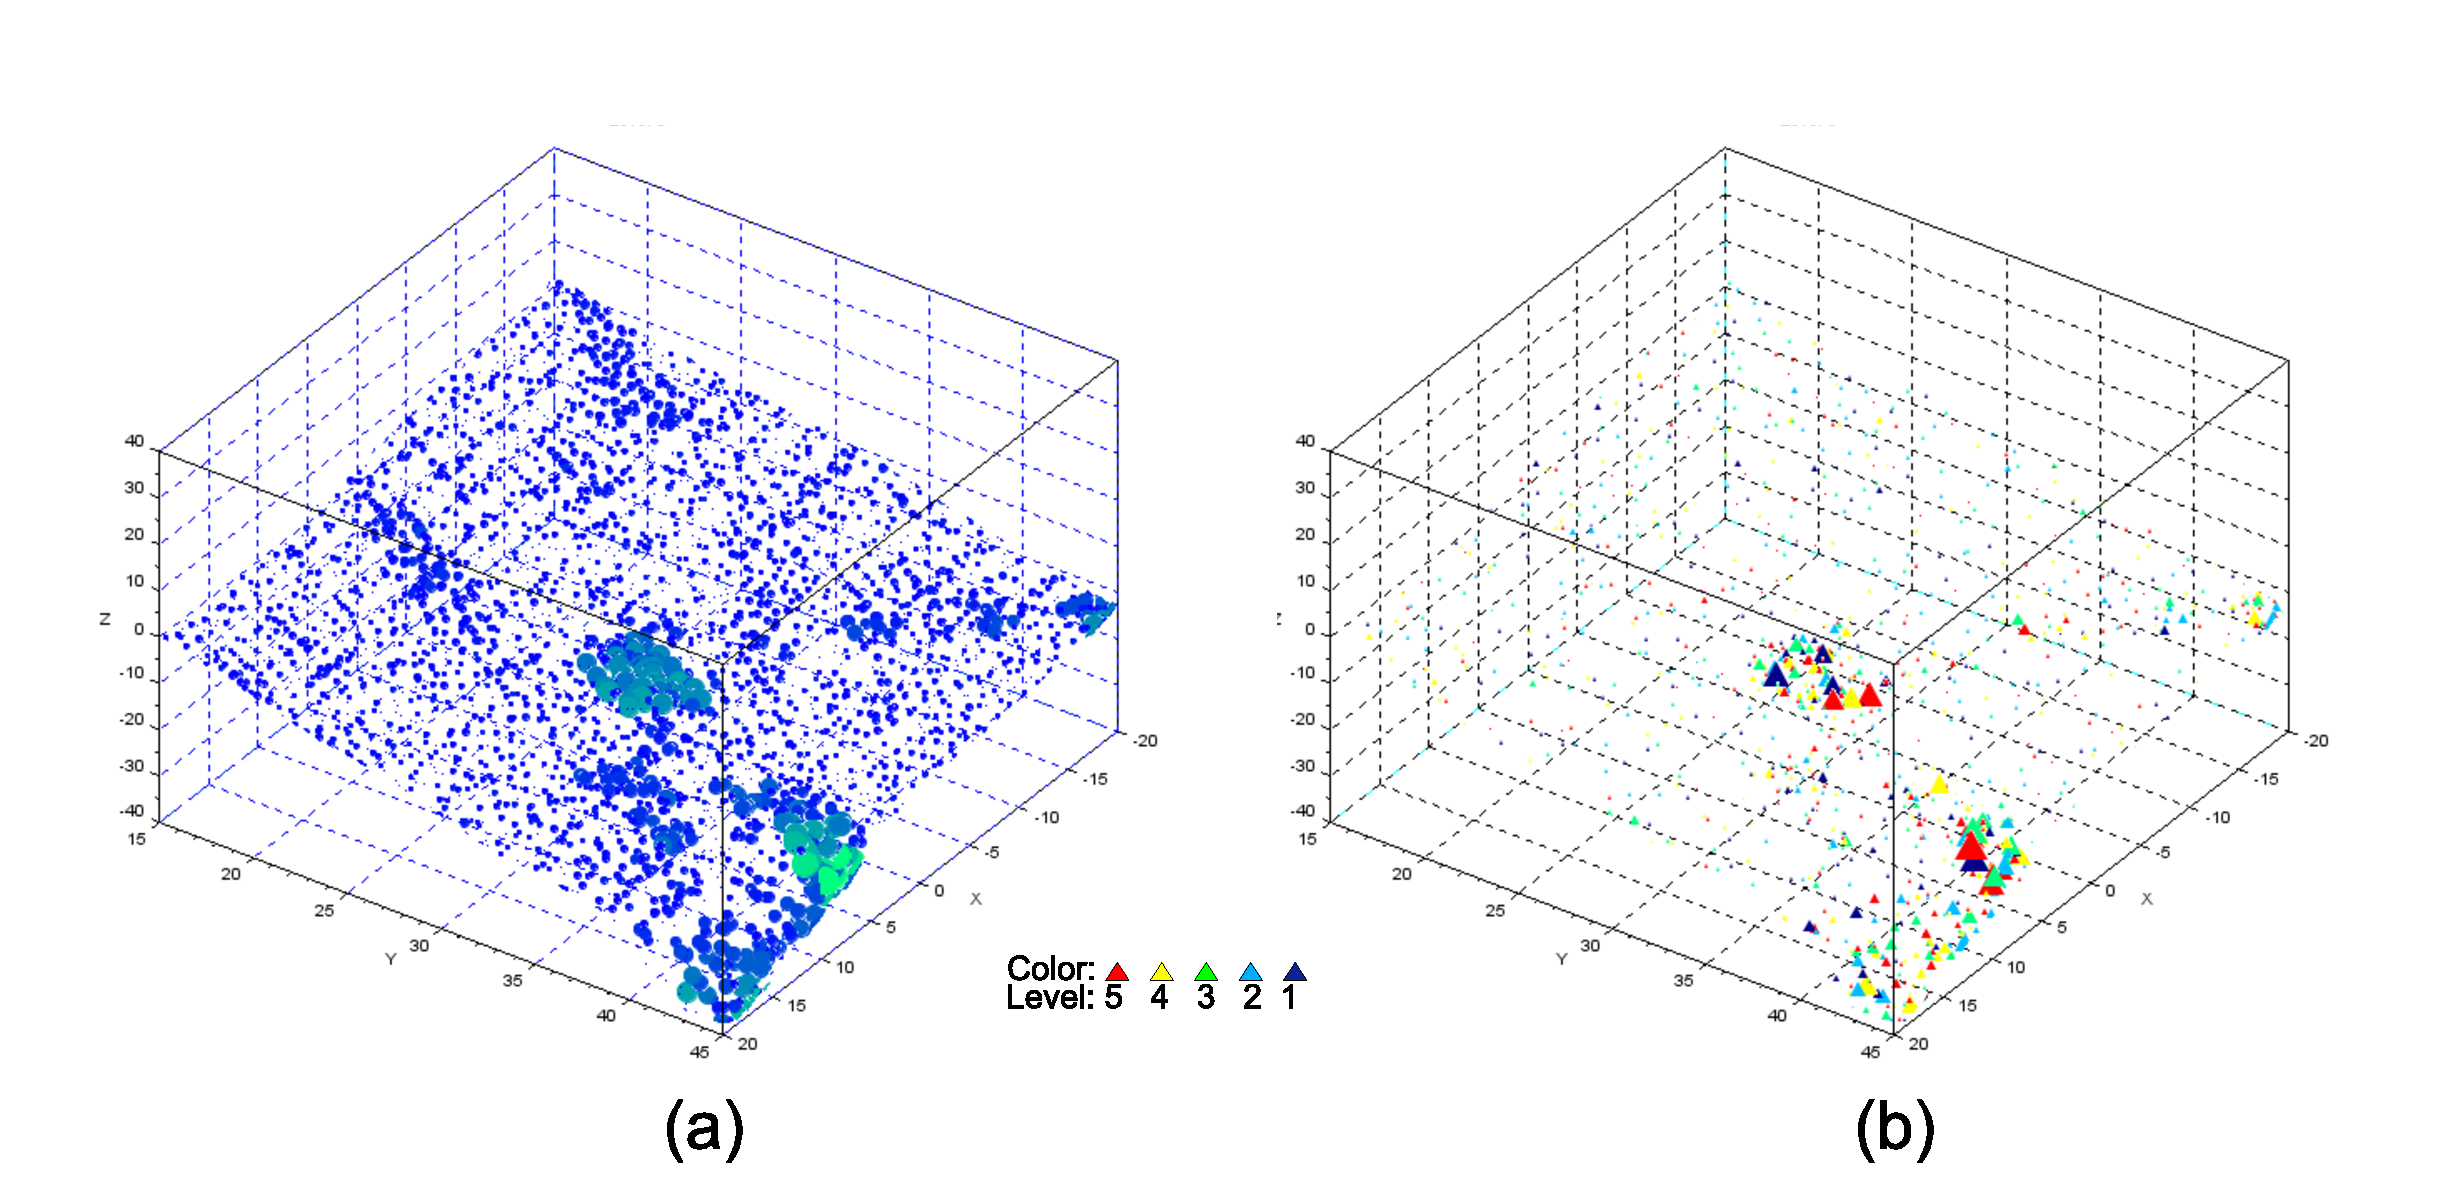
\includegraphics[width=1\linewidth]{figs/KauaiVFA.pdf}
		%
		\caption{\label{fig_cds:diff_vector_5}
			Difference vector magnitude across 5 consecutive analysis passes of the Kauai fragment \ref{fig_cds:Kauai}. The (a) subplot reveals the height above ground of the initial terrain points, while the (b) subplot contains markers indicating the strength (size) and frequency band of the resulting difference vectors at each of the odd vertices present in the (a) subplot. The regions in (a) with abrupt variations register a high frequency footprint, while similar points clustered together register lower frequency signatures as well. }
	\end{figure}
	
	\subsection{Discussion and conclusions}
	Several conclusions can be drawn by analyzing the results obtained using the different lifting designs. First, by using the update designs that are not guaranteed to preserve the signal average for general graphs (e.g. \cite{ Martinez2011}), we observe the RMSE levels have the highest values, regardless of the prediction filter design. As such, the charts \ref{fig_cds:smokey_lod_rmse}a, \ref{fig_cds:fundata_lod_rmse}a and \ref{fig_cds:iezer_lod_rmse}a reveal that over a progression of 12 analysis steps, the uniform weighing prediction design (\textbf{UG}) is, on average, the better choice. While the geometric Laplacian (\textbf{GL}) and the non-negative least squares weights (\textbf{NNLS}) yield better quality results, after  6 or 7 decomposition steps they become unstable. The use of the cotangent Laplacian weights (\textbf{CL}) is not justified either, since this design takes into account only the geometric structure of the data, regardless of the attribute variability. Overall, both uniform and cotangent Laplacian weights produce more stable results, but the uniform design is to be preferred due to its consistently lower RMSE levels. Next, directly preserving the average of the scale coefficients in a one-ring neighborhood (\textbf{ORMP}) contributes to both  stability and error-minimizing properties of the analysis sequence for all sets (charts \ref{fig_cds:smokey_lod_rmse}b, \ref{fig_cds:fundata_lod_rmse}b and \ref{fig_cds:iezer_lod_rmse}b). The best results are, however, achieved through the use of the minimum norm, mean preserving update weights (proposed by Jansen et al. \cite{Jansen2001}). This design ensures the highest stability while sensibly decreasing the mean square error. More specifically, for all terrain sets the \textbf{ORMP} design is surpassed by the combined use of Laplacian prediction weights and the minimum norm update vector coefficients. Both of our proposals, the geometric Laplacian (\textbf{GLMN}) and the non-negative least squares (\textbf{NNLSMN}) attain an almost twofold accuracy over the cotangent (\textbf{CLMN}) and uniform weights Laplacian (\textbf{UGMN}). While the RMSE could be reduced even further by lifting the constraints on the least squares prediction filter, as proposed in \cite{Wagner2005} and in \cite{Martinez2011}, the scheme becomes numerically unstable due to both the potentially very high values of the weights and the prediction of the boundary vertices. While we can fix the boundary vertices and alleviate the stability issue, our design does not require such vertex selection constraints to be applied.
	
	The multiresolution experiments conducted with the three samples also confirm the 25\% reduction ratio of the number of vertices after each downsampling step. More specifically, the average reduction rate attained for the Smoky set (figure \ref{fig_cds:smokey_lod_rmse}) is 27\%, for the high-density Carpathian set (figure \ref{fig_cds:fundata_lod_rmse}) the average ratio is 28\%, and for the low-density Carpathian set (figure \ref{fig_cds:iezer_lod_rmse})  this average ratio is 27\%.
	
	As immediate applications for this graph-wavelet multiresolution framework, we suggest filtering \cite{CDS2017} and, as experimentally examined in figure \ref{fig_cds:diff_vector_5}, we also suggest considering the potential of using the detail vector information to offer an intuitive classification similar to that of vertex frequency analysis.
	
	
	%%%%%%%%%%%%%%%%%%%%%%%%%%%%%%%%%%%%%%%%%%%%%%%%%
	
	
	
	
	% Use the \index{} command to code your index words
	%
	%
	
	
	%\begin{acknowledgement}
		
	%\end{acknowledgement}
	%
	
	%%%%%%%%%%%%%%%%%%%%%%%% referenc.tex %%%%%%%%%%%%%%%%%%%%%%%%%%%%%%
% sample references
% %
% Use this file as a template for your own input.
%
%%%%%%%%%%%%%%%%%%%%%%%% Springer-Verlag %%%%%%%%%%%%%%%%%%%%%%%%%%
%
% BibTeX users please use
% \bibliographystyle{}
% \bibliography{}
%
\biblstarthook{References may be \textit{cited} in the text either by number (preferred) or by author/year.\footnote{Make sure that all references from the list are cited in the text. Those not cited should be moved to a separate \textit{Further Reading} section or chapter.} The reference list should ideally be \textit{sorted} in alphabetical order -- even if reference numbers are used for the their citation in the text. If there are several works by the same author, the following order should be used: 
}

\begin{thebibliography}{99}
	
	\bibitem{AbdulRahman2013}
	Hussein~S. Abdul-Rahman, Xiangqian~Jane Jiang, and Paul~J. Scott.
	\newblock Freeform surface filtering using the lifting wavelet transform.
	\newblock {\em Precision Engineering}, 37(1):187 -- 202, 2013.
	
	\bibitem{Bertram2007}
	Martin Bertram.
	\newblock Wavelet analysis for progressive meshes.
	\newblock In {\em Proceedings of the 23rd Spring Conference on Computer
		Graphics}, SCCG '07, pages 161--167, New York, NY, USA, 2007. ACM.
	
	\bibitem{Beyer2003}
	G.~Beyer.
	\newblock Terrain inclination and curvature from wavelet coefficients.
	\newblock {\em Journal of Geodesy}, 76(9):557--568, 2003.
	
	\bibitem{Chen2010}
	Guangliang Chen and M.~Maggioni.
	\newblock Multiscale geometric wavelets for the analysis of point clouds.
	\newblock In {\em Information Sciences and Systems (CISS), 2010 44th Annual
		Conference on}, pages 1--6, March 2010.
	
	\bibitem{Choi2005}
	Hyeokho Choi and R.~Baraniuk.
	\newblock Multiscale manifold representation and modeling.
	\newblock In {\em Acoustics, Speech, and Signal Processing, 2005. Proceedings.
		(ICASSP '05). IEEE International Conference on}, volume~4, pages
	iv/569--iv/572 Vol. 4, March 2005.
	
	\bibitem{Cioaca2016UPB}
	Teodor Cioaca, Bogdan Dumitrescu, and Mihai-Sorin Stupariu.
	\newblock Combined quadric error metric and lifting scheme multivariate model
	simplification.
	\newblock {\em U.P.B. Scientific Bulletin, series C}, 2016.
	
	\bibitem{Cioaca2016}
	Teodor Cioaca, Bogdan Dumitrescu, and Mihai-Sorin Stupariu.
	\newblock Graph-based wavelet representation of multi-variate terrain data.
	\newblock {\em Computer Graphics Forum}, 35(1):44--58, 2016.
	
	\bibitem{Cioaca2016CEAI}
	Teodor Cioaca, Bogdan Dumitrescu, and Mihai-Sorin Stupariu.
	\newblock Lazy wavelet simplification using scale-dependent dense geometric
	variability descriptors.
	\newblock {\em Journal of Control Engineering and Applied Informatics}, 2016.
	
	\bibitem{CDS2017}
	Teodor Cioaca, Bogdan Dumitrescu, and Mihai{-}Sorin Stupariu.
	\newblock Riemannian filters for multi-variate mesh signals.
	\newblock In {\em Proceedings of the 12th International Joint Conference on
		Computer Vision, Imaging and Computer Graphics Theory and Applications
		{(VISIGRAPP} 2017) - Volume 1: GRAPP, Porto, Portugal, February 27 - March 1,
		2017.}, pages 228--235, 2017.
	
	\bibitem{Cioaca2015}
	Teodor Cioaca, Bogdan Dumitrescu, Mihai-Sorin Stupariu, and et~al.
	\newblock Heuristic-driven graph wavelet modeling of complex terrain.
	\newblock In Yulin Wang; Xudong Jiang;~David Zhang, editor, {\em Sixth
		International Conference on Graphic and Image Processing (ICGIP 2014)},
	volume 9443. SPIE Proceedings, 3 2015.
	
	\bibitem{Coifman2006}
	Ronald~R. Coifman and Mauro Maggioni.
	\newblock Diffusion wavelets.
	\newblock {\em Applied and Computational Harmonic Analysis}, 21(1):53 -- 94,
	2006.
	\newblock Special Issue: Diffusion Maps and Wavelets.
	
	\bibitem{Demaret2005}
	Laurent Demaret, Nira Dyn, Michael~S. Floater, and Armin Iske.
	\newblock Adaptive thinning for terrain modelling and image compression.
	\newblock In Neil~A. Dodgson, Michael~S. Floater, and Malcolm~A. Sabin,
	editors, {\em Advances in Multiresolution for Geometric Modelling}, pages
	319--338, Berlin, Heidelberg, 2005. Springer Berlin Heidelberg.
	
	\bibitem{Evans2007}
	J.~S. Evans and A.~T. Hudak.
	\newblock A multiscale curvature algorithm for classifying discrete return
	lidar in forested environments.
	\newblock {\em IEEE Transactions on Geoscience and Remote Sensing},
	45(4):1029--1038, April 2007.
	
	\bibitem{Floriani2016}
	Leila~De Floriani and Paola Magillo.
	\newblock {\em Triangulated Irregular Network}, pages 1--2.
	\newblock Springer New York, New York, NY, 2016.
	
	\bibitem{Fujiwara95}
	K~Fujiwara.
	\newblock Eigenvalues of laplacians on a closed riemannian manifold and its
	nets.
	\newblock In Proceedings of AMS 123, 1995.
	
	\bibitem{Garland1998}
	Michael Garland and Paul~S. Heckbert.
	\newblock Simplifying surfaces with color and texture using quadric error
	metrics.
	\newblock In {\em Proceedings of the Conference on Visualization '98}, VIS '98,
	pages 263--269, Los Alamitos, CA, USA, 1998. IEEE Computer Society Press.
	
	\bibitem{Guskov1999}
	Igor Guskov, Wim Sweldens, and Peter Schr\"{o}der.
	\newblock Multiresolution signal processing for meshes.
	\newblock In {\em Proceedings of the 26th Annual Conference on Computer
		Graphics and Interactive Techniques}, SIGGRAPH '99, pages 325--334, New York,
	NY, USA, 1999. ACM Press/Addison-Wesley Publishing Co.
	
	\bibitem{Hammond2011}
	David~K. Hammond, Pierre Vandergheynst, and R�mi Gribonval.
	\newblock Wavelets on graphs via spectral graph theory.
	\newblock {\em Applied and Computational Harmonic Analysis}, 30(2):129 -- 150,
	2011.
		
	\bibitem{Isenburg2015}
	M~Isenburg.
	\newblock Lastools--efficient tools for lidar processing, version 150304, 2015.
	
	\bibitem{Jansen2013}
	M.~Jansen.
	\newblock Multiscale local polynomial smoothing in a lifted pyramid for
	non-equispaced data.
	\newblock {\em Signal Processing, IEEE Transactions on}, 61(3):545--555, Feb
	2013.
	
	\bibitem{Jansen2001}
	MH~Jansen, GP~Nason, and BW~Silverman.
	\newblock {\em Scattered data smoothing by empirical Bayesian shrinkage of
		second generation wavelet coefficients}, volume 4478.
	\newblock 2001.
	\newblock Other: M Unser and A Aldroubi, (eds).
	
	\bibitem{Jestrovic2017}
	Iva Jestrovi\'c, James~L. Coyle, and Ervin Sejdi\'c.
	\newblock A fast algorithm for vertex-frequency representations of signals on
	graphs.
	\newblock {\em Signal Processing}, 131:483 -- 491, 2017.
	
	\bibitem{Kalbermatten2012}
	Michael Kalbermatten, Dimitri Van~De Ville, Pascal Turberg, Devis Tuia, and
	Stephane Joost.
	\newblock Multiscale analysis of geomorphological and geological features in
	high resolution digital elevation models using the wavelet transform.
	\newblock {\em Geomorphology}, 138(1):352 -- 363, 2012.
	
	\bibitem{Lounsbery1994}
	Michael Lounsbery.
	\newblock {\em Multiresolution Analysis for Surfaces of Arbitrary Topological
		Type}.
	\newblock PhD thesis, Dept. of Computer Science and Engineering, U. of
	Washington, 1994.
	
	\bibitem{Martinez2011}
	E.~Martinez-Enriquez and A.~Ortega.
	\newblock Lifting transforms on graphs for video coding.
	\newblock In {\em Data Compression Conference (DCC), 2011}, pages 73--82, 2011.
	
	\bibitem{Meyer2003}
	Mark Meyer, Mathieu Desbrun, Peter Schr�der, and AlanH. Barr.
	\newblock Discrete differential-geometry operators for triangulated
	2-manifolds.
	\newblock In Hans-Christian Hege and Konrad Polthier, editors, {\em
		Visualization and Mathematics III}, Mathematics and Visualization, pages
	35--57. Springer Berlin Heidelberg, 2003.
	
	\bibitem{Pauly2002}
	Mark Pauly, Markus Gross, and Leif~P. Kobbelt.
	\newblock Efficient simplification of point-sampled surfaces.
	\newblock In {\em Proceedings of the Conference on Visualization '02}, VIS '02,
	pages 163--170, Washington, DC, USA, 2002. IEEE Computer Society.
	
	\bibitem{Payan2006}
	Frederic Payan and Marc Antonini.
	\newblock Mean square error approximation for wavelet-based semiregular mesh
	compression.
	\newblock {\em IEEE Transactions on Visualization and Computer Graphics},
	12(4):649--657, July 2006.
	
	\bibitem{Ronfard1996}
	R�mi Ronfard and Jarek Rossignac.
	\newblock Full-range approximation of triangulated polyhedra.
	\newblock {\em Computer Graphics Forum}, 15(3):67--76, 1996.
	
	\bibitem{Schroeder1992}
	William~J. Schroeder, Jonathan~A. Zarge, and William~E. Lorensen.
	\newblock Decimation of triangle meshes.
	\newblock {\em SIGGRAPH Comput. Graph.}, 26(2):65--70, July 1992.
	
	\bibitem{Shuman2016}
	David~I Shuman, Benjamin Ricaud, and Pierre Vandergheynst.
	\newblock Vertex-frequency analysis on graphs.
	\newblock {\em Applied and Computational Harmonic Analysis}, 40(2):260 -- 291,
	2016.
	
	\bibitem{Silva2018}
	Carlos~Alberto Silva, Carine Klauberg, Angela Maria~Klein Hentz, Ana
	Paula~Dalla Corte, Uelison Ribeiro, and Veraldo Liesenberg.
	\newblock {Comparing the Performance of Ground Filtering Algorithms for Terrain
		Modeling in a Forest Environment Using Airborne LiDAR Data}.
	\newblock {\em {Floresta e Ambiente}}, 25, 00 2018.
	
	\bibitem{Suarez2009}
	J.P. Su�rez and A.~Plaza.
	\newblock Four-triangles adaptive algorithms for rtin terrain meshes.
	\newblock {\em Mathematical and Computer Modelling}, 49(5):1012 -- 1020, 2009.
	
	\bibitem{Sweldens1996}
	Wim Sweldens.
	\newblock The lifting scheme: A custom-design construction of biorthogonal
	wavelets.
	\newblock {\em Applied and Computational Harmonic Analysis}, 3(2):186 -- 200,
	1996.
	
	\bibitem{vanKreveld1997}
	Marc van Kreveld.
	\newblock Digital elevation models and tin algorithms.
	\newblock In {\em Algorithmic foundations of geographic information systems},
	pages 37--78. Springer, 1997.
	
	\bibitem{Wagner2005}
	R.~Wagner, Hyeokho Choi, R.~Baraniuk, and V.~Delouille.
	\newblock Distributed wavelet transform for irregular sensor network grids.
	\newblock In {\em Statistical Signal Processing, 2005 IEEE/SP 13th Workshop
		on}, pages 1196--1201, 2005.
	
	\bibitem{Wardetzky2007}
	Max Wardetzky, Saurabh Mathur, Felix K\"{a}lberer, and Eitan Grinspun.
	\newblock Discrete laplace operators: No free lunch.
	\newblock In {\em Proceedings of the Fifth Eurographics Symposium on Geometry
		Processing}, SGP '07, pages 33--37, Aire-la-Ville, Switzerland, Switzerland,
	2007. Eurographics Association.
	
	\bibitem{WuA03}
	Jingsong Wu and Kevin Amaratunga.
	\newblock Wavelet triangulated irregular networks.
	\newblock {\em International Journal of Geographical Information Science},
	17(3):273--289, 2003.
	
\end{thebibliography}


\end{document}
